\chapter{Fully Neuromorphic Vision and Control for Autonomous Drone Flight}
\label{cha:sr}

{\it
Fede still had this at the non-final version, so there are quite some changes.
}

\blfootnote{The contents of this chapter have been published in:\\
	\vspace{-10pt}\begin{blockquote}
	F.\ Paredes-Vall\'es$^\dagger$, \textbf{J.\ J.\ Hagenaars}$^\dagger$, J.\ D.\ Dupeyroux$^\dagger$, S.\ Stroobants, Y.\ Xu, G.\ C.\ H.\ E.\ de Croon, \emph{Fully neuromorphic vision and control for autonomous drone flight}, Science Robotics, 2023.
\end{blockquote}%\vspace{-10pt}
Although not covered in this dissertation, this chapter also builds on the following publications:\\
\vspace{-10pt}\begin{blockquote}
	J.\ D.\ Dupeyroux, \textbf{J.\ J.\ Hagenaars}, F.\ Paredes-Vall\'es, G.\ C.\ H.\ E.\ de Croon, \emph{Neuromorphic control for optic-flow-based landing of MAVs using the Loihi processor}, IEEE International Conference on Robotics and Automation (ICRA), 2021.\\
	\textbf{J.\ J.\ Hagenaars}, F.\ Paredes-Vall\'es, G.\ C.\ H.\ E.\ de Croon, \emph{Evolved neuromorphic control for high speed divergence-based landings of MAVs}, IEEE Robotics and Automation Letters (RA-L), 2020.
\end{blockquote}%\vspace{-10pt}
{\scriptsize$\dagger$~~Equal contribution.}\\
$\text{}$\\
\textbf{Contribution:} The research in this chapter was a collaborative effort with multiple researchers, all from the Micro Air Vehicle Laboratory (Delft University of Technology). We all contributed equally to the conception of the study, to performing the experiments, and to the analysis of the results. My main contribution lay in the design and implementation of the control pipeline. This involved training neural control in simulation, designing the interface with the vision-based state estimation, and ensuring a successful sim-to-real transfer.
}

\newpage
\thispagestyle{empty}
\phantom{blabla}
\newpage

\section{Introduction}

\dropcap{O}ver the past decade, deep artificial neural networks (ANNs) have revolutionized the field of artificial intelligence. Among the successes has been the substantial improvement of visual processing, to an extent that computer vision can now outperform humans on specific tasks \cite{ciresan2011committee}. Also the field of robotics has benefited from this development, with deep ANNs achieving state-of-the-art accuracy in tasks such as stereo vision \cite{cheng2020hierarchicala,gu2020cascadea}, optical flow estimation \cite{ilg2017flowneta,sun2018pwcnet,teed2020rafta}, segmentation \cite{yuan2021segmentation,liu2022swina}, object detection \cite{girshick2015fasta,redmon2018yolov3a,xu2021endtoend}, and monocular depth estimation \cite{garg2016unsuperviseda,godard2017unsuperviseda,yuan2022newa}.
However, this high accuracy typically relies on substantial neural network sizes that require quite heavy and power-hungry processing hardware (tens of watts, hundreds of grams~\cite{nvidia}). This limits the number of tasks that can be performed by larger (ground) robots, and even prevents deployment on smaller robots with highly stringent resource constraints, like small flying drones. 

Neuromorphic hardware may provide a solution to this problem, since it mimics the energy-efficient, sparse and asynchronous nature of sensing and processing in biological brains~\cite{indiveri2000neuromorphica,sandamirskaya2022neuromorphic}. For example, the pixels in neuromorphic, event-based cameras only transmit information on brightness changes \cite{gallego2020eventbased}. Since typically only a fraction of the pixels change in brightness substantially, this leads to sparse vision inputs with subsequent events that are in the order of a microsecond apart. The asynchronous and sparse nature of visual inputs from event-based cameras represents a paradigm shift compared to traditional, frame-based computer vision. Ideally, processing would exploit these properties for quicker, more energy-efficient processing. However, currently, learning-based approaches to event-based vision involve accumulating events over a substantial amount of time, creating an ``event window'' that represents extended temporal information. This window is then processed similarly to a traditional image frame with an ANN \cite{zhu2018evflownet,zhu2019unsuperviseda,gehrig2021eraft,paredes-valles2021back}.
Although there is work that employs much shorter event windows \cite{paredes-valles2020unsupervised,hagenaars2021selfsupervised, paredes2023taming}, latency could be further reduced by processing events asynchronously as they come in. This could be performed by neuromorphic processors designed for implementing spiking neural networks (SNNs) \cite{maass1997networksa,gruning2014spikinga}. These networks have temporal dynamics more similar to biological neurons. In particular, the neurons have a membrane voltage that integrates incoming inputs and causes a spike when it exceeds a threshold. The binary nature of spikes allows for more energy-efficient processing than the floating point arithmetic in traditional ANNs \cite{davies2021advancing,ottati2023spikea}. The energy gain is further improved by reducing the spiking activity as much as possible, as is also a main property of biological brains \cite{sterling2015principlesa}. Coupling neuromorphic vision to neuromorphic processing promises low-energy and low-latency visual sensing and acting, as exhibited by agile animals such as flying insects \cite{muijres2014fliesa}.

However, in order to achieve these properties, several challenges have to be overcome related to present-day neuromorphic sensing and processing. For example, training is currently still much more difficult for SNNs than for ANNs \cite{pfeiffer2018deepa,tavanaei2019deepa}, mostly due to their sparse, binary, and asynchronous nature. The most well-known difficulty of SNN learning is the non-differentiability of the spiking activation function, which prevents naive application of backpropagation. Currently, this is tackled rather successfully with the help of surrogate gradients \cite{neftci2019surrogatea,zenke2021remarkable}, although longer sequences (as would be the case for event-by-event processing) can still lead to gradient vanishing. Moreover, although the richer neural dynamics can potentially represent more complex temporal functions, they are also harder to shape; and neural activity may saturate or dwindle during training, preventing further learning. The causes for this are hard to analyze, as there are many parameters that can play a role. Depending on the model, the relevant parameters may range from neural leaks and thresholds to recurrent weights and time constants for synaptic traces. A solution may lie in learning these parameters \cite{chowdhury2021understanding,fang2021incorporating}, but this further increases the dimensionality of the learning problem. Finally, when targeting a robotics application, SNN training and deployment is further complicated by the restrictions of existing embedded neuromorphic processing platforms. These restrictions were recently highlighted in a study on neuromorphic route learning \cite{zhu2023neuromorphic}, and include hardware and software challenges such as interfacing with neuromorphic cameras, the limitations of available neural models and\textemdash importantly\textemdash the still rather limited numbers of available neurons and synapses. To illustrate this latter point, the ROLLS chip~\cite{qiao2015reconfigurable} accommodates 256 spiking neurons, the Intel Kapoho Bay (featuring two Loihi chips \cite{davies2018loihi} in a USB stick form factor) features 262,100 neurons \cite{vitale2021eventdriven}, and the SpiNNaker version in \cite{galluppi2014eventbased} has 768,000 neurons. Although these chips differ in many more aspects than only the  number of neurons, this small sample already shows that current state-of-the-art SNNs cannot be easily embedded on robots. SNNs that have recently been trained on visually complex tasks such as optical flow determination \cite{paredes-valles2020unsupervised,hagenaars2021selfsupervised} still feature far too large network sizes for implementation on current neuromorphic processing hardware for embedded systems. The smallest size SNN in these studies is LIF-FireFlowNet (Leaky-Integrate and Fire) for optical flow estimation \cite{hagenaars2021selfsupervised}, which still has 3.7 million neurons (at an input resolution of 128$\times$128 pixels).

As a consequence, pioneering work in this area has been limited in complexity. Very early work involved the evolution of spiking neural network connectivity to map the 16 visual brightness inputs of a wheeled Kephera robot to its two motor outputs \cite{floreano2001evolution}. The evolved SNN, simulated in software, allowed the robot to avoid the walls in a black-and-white-striped environment. Most work exploring SNNs for robotic vision focuses on simulation. For example, in \cite{bing2018enda}, the events from a simulated event-based camera with 128$\times$128 pixels are accumulated into frames, compressing them over time into 8$\times$4 Poisson input neurons. These inputs, which capture the clear white lines of the road border, are then directly mapped to two output neurons for staying in the center of the road with the help of reward-modulated spike-time-dependent plasticity  learning. Robotic examples of in-hardware neuromorphic processing for vision are more rare. An early example is the one in \cite{galluppi2014eventbased}, in which an event-based camera with 128$\times$128 pixels is connected to a SpiNNaker neuromorphic processor to allow a driving robot to differentiate between two lights flashing at different frequencies with a 128-neuron winner-takes-all network. In \cite{milde2017obstacle} a spiking neural network is designed for following a light target in the top half of the field of view, while avoiding regions with many events in the bottom half of the field of view. This network is successfully implemented in the ROLLS neuromorphic chip~\cite{qiao2015reconfigurable} and tested in an office environment. Recent years have seen an increasing focus on flying robots (drones), because they need to react quickly while being extremely restricted in terms of size, weight, and power (SWaP). In \cite{vitale2021eventdriven}, an SNN is implemented on a bench-fixed dual-rotor to align the roll angle with a black-and-white disk located in front of the camera. The SNN involved both a visual Hough transform \cite{ballard1981generalizinga} for finding the line, and a proportional-derivative (PD) controller for generating the propeller commands. Finally, in \cite{dupeyroux2021neuromorphica}, an SNN was first evolved in simulation and then implemented in Loihi for vision-based landing of a flying drone. This control network only consisted of 35 neurons since the visual processing was still performed with conventional, frame-based computer vision methods. Additionally, it is worth noting that only the vertical motion of the drone was controlled with the SNN; its lateral position was controlled using traditional control algorithms and an external motion capture system. The current work represents a step up in complexity by performing three-dimensional visual ego-motion estimation and control of a flying drone with a fully neuromorphic vision-to-control pipeline.

In this chapter, we present a fully neuromorphic vision-to-control pipeline for controlling a flying drone, demonstrating the potential of neuromorphic hardware. The presented pipeline consists of a spiking neural network that is trained to accept raw event-camera data and output low-level control actions for performing autonomous vision-based ego-motion estimation and control at approximately 200 Hz. A core property of our learning setup is that it splits vision and control, which provides two major advantages. First, it helps to prevent the reality gap on the camera event input side, as the vision part is trained based on the raw events from the actual event camera on the drone. We use self-supervised learning, since this foregoes the need for ground truth measurements that are difficult to obtain for event-based vision. Second, as the output of the vision part is an ego-motion estimate, we can learn the control in a simple and extremely fast simulator. This allows us to evade the high-frequency generation of visually realistic images for event generation \cite{rebecq2018esim}, something that would lead to excessive training times in an end-to-end learning setup. 

\begin{figure*}[!t]
	\centering
	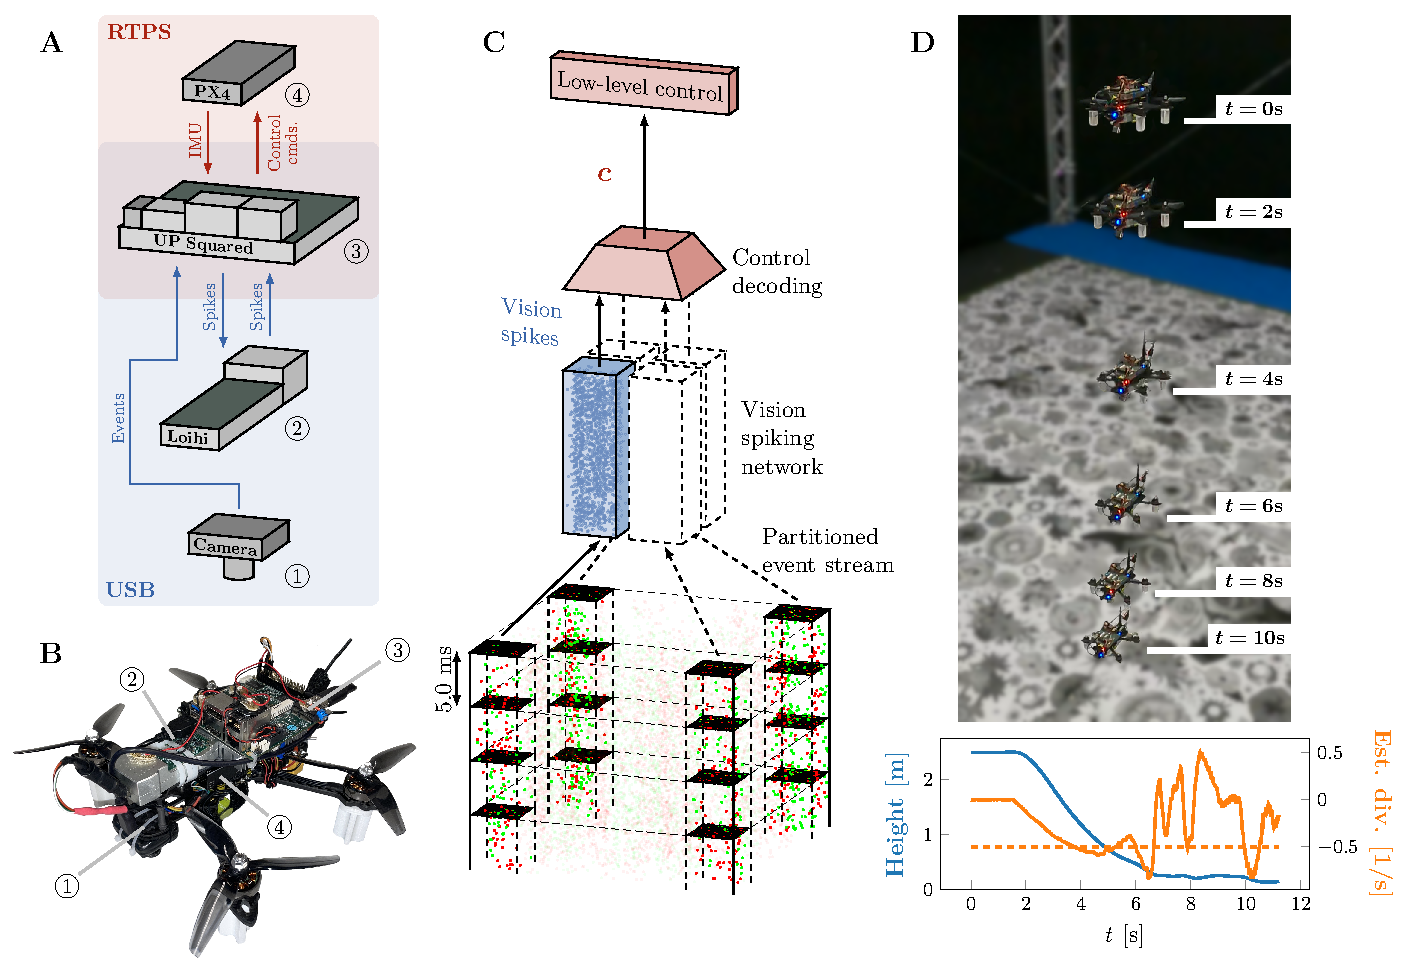
\includegraphics[width=\textwidth]{04_chapters/SR23/figures/fig1-pipeline.pdf}
	\caption{Overview of the proposed system. (\textit{A}) Hardware overview showing the communication between event-camera, neuromorphic processor, single-board computer and flight controller. RTPS (real-time publish-subscribe) and USB refer to the used communication protocols. (\textit{B}) Quadrotor used in this work (total weight 994 g, tip-to-tip diameter 35 cm). (\textit{C}) Pipeline overview showing events as input, processing by the vision network and decoding into a control command. (\textit{D}) Demonstration of the system for an optical flow constant divergence landing.} \label{fig:sr_pipeline}
\end{figure*}

\subsection*{A fully neuromorphic solution to vision-based navigation}

The fully neuromorphic vision-to-control pipeline, illustrated in \figref{fig:sr_pipeline}C, was implemented on the Loihi neuromorphic processor~\cite{davies2018loihi} and used on board a small flying robot (see \figref{fig:sr_pipeline}B) for vision-based navigation. A schematic of the hardware setup employed is shown in \figref{fig:sr_pipeline}A. The system successfully followed ego-motion setpoints (target values) in a fully autonomous fashion, without any external aids such as a positioning system. \figref{fig:sr_pipeline}D shows an example of a landing experiment with our neuromorphic pipeline in the control loop of the drone.
The figure shows the smoothly decreasing height of the drone above the ground (blue line), and the estimated optical flow divergence (orange line), which is the vertical component of the velocity vector divided by this height. The divergence curve is typical of an optical flow divergence landing, first approaching the setpoint -0.5~1/s and then becoming more oscillatory when getting very close to the ground~\cite{decroon2016monocular}.

As mentioned, the main challenge of deploying such a pipeline on embedded neuromorphic hardware is that, due to the preliminary state of this technology, one has to work within very tight limits regarding the available computational resources. In this project, several design decisions were made to adapt to these limitations. Firstly, the vision processing pipeline assumes that the event-based camera on the drone, the DVS 240~\cite{brandli2014240a}, looks down at a static, texture-rich, flat surface. Knowing the structure of the visual scene in advance simplifies the estimation of the ego-motion of the camera (and hence of the drone) with the help of optical flow information, as in \cite{decroon2013opticflow,decroon2016monocular,pijnackerhordijk2018vertical,hagenaars2020evolveda,dupeyroux2021neuromorphica}. Optical flow, or the apparent motion of scene points in the image space, can be estimated from the output of an event-based camera with a wide variety of methods, ranging from sparse feature-tracking algorithms \cite{benosman2012asynchronousa} to dense (per-pixel) machine learning models \cite{zhu2018evflownet,gehrig2021eraft,hagenaars2021selfsupervised}. In the search for an efficient and high-bandwidth vision pipeline that achieves the desired 200~Hz operating frequency, the second design decision was to reduce the spatial resolution of the event-based vision data by only processing information from the image corner regions of interest (ROIs) rather than the entire image space, and to limit the number of events to 90 per ROI. More specifically, as depicted in \figreftwo{fig:pipeline}{C}{fig:vision}{A}, we propose the use of a small spiking neural network that is applied independently at each ROI, with each ROI being 16$\times$16 pixels in size after a nearest-neighbor downsampling operation. Each network consists of 7,200 neurons and 506,400 synapses distributed over five spiking layers: one input layer, three self-recurrent encoders, and a pooling layer. Its parameters (weights, thresholds, and leaks) are identical for the four ROIs, and it estimates the optical flow, in pixels per millisecond, of the corresponding ROI.
Because of the static and planar scene assumption, the apparent motion of the scene points at the four corner ROIs encodes non-metric information about the velocity of the camera (divided by the distance to the surface along the optical axis) and its rotational rates in a linear manner \cite{baker2006parameterizing}.

\begin{figure*}[!t]
	\centering
	\includegraphics[width=\textwidth]{04_chapters/SR23/figures/fig2-vision.pdf}
	\caption{Overview of the spiking vision network. Running at approx. 200~Hz, events are accumulated (max.\ 90 events per corner ROI) and then fed through the vision network consisting of three encoders (kernel size $3\times3$, stride 2) and a spiking pooling layer. Spikes are decoded into two floats representing flow for that corner ROI. This network is replicated to the three other ROIs, in order to end up with four ROI optical flows vectors. During training, these are used in a homography transformation to derive dense flow, which is then used for the self-supervised loss. The full network is running on the neuromorphic processor during real-world flight tests.}
	\label{fig:sr_vision}
\end{figure*}

Based on this information, the robot performs ego-motion control. To keep the pipeline fully neuromorphic (minimum required processing happening outside of Loihi) and performant (sending more spikes to Loihi decreases execution frequency), we trained a linear controller in simulation, and merged it with the decoding of the spikes coming from the vision network (representing optical flow). In other words, the linear controller takes vision spikes, a user-given ego-motion setpoint, and attitude of the drone and maps these linearly to thrust and attitude control commands. Although opting for a linear controller allows for a fully neuromorphic vision-to-control pipeline, it also means we had to make some assumptions. For instance, angles in pitch and roll should be small, and the optical flow variables taken as input should be derotated in pitch and roll \cite{decroon2013opticflow,longuet-higgins1980interpretation}. Furthermore, we should keep in mind that a linear controller will be unable to compensate for any drift or steady-state offset through integration (as could be done by a common proportional integral derivative or PID controller). We show that, despite all this, we can successfully control a flying drone to perform certain ego-motion maneuvers.

We split the training of our vision-to-control pipeline into two separate frameworks. On the one hand, the vision part of the pipeline, in charge of mapping input events to optical flow, was trained in a self-supervised fashion using the contrast maximization framework \cite{gallego2018unifying,gallego2019focusa}. The idea behind this approach is that, by compensating for the spatiotemporal misalignments among the events triggered by a moving edge (event deblurring), one can retrieve accurate optical flow information. In this work, we used the formulation proposed in \cite{hagenaars2021selfsupervised} and shown in \figref{fig:vision}. Corner ROI events within non-overlapping temporal windows of five milliseconds are processed sequentially by our spiking networks, which provide optical flow estimates at every timestep. Only during training, we have used the motion information of the four corner ROIs to parameterize a homography transformation that, under the assumption of static planar surface, allowed us to retrieve dense optical flow, as in \cite{baker2006parameterizing, detone2016deep, nguyen2018unsupervised, sanket2020evdodgeneta}. Following \cite{hagenaars2021selfsupervised}, we have accumulated event and optical flow tuples over multiple timesteps for contrast maximization to be a robust self-supervisory signal, and only computed the deblurring loss function and performed a backward pass through the networks (using backpropagation through time) once 25 milliseconds of event data were processed. To cope with the non-differentiable spiking function of our neurons, we have used surrogate gradients \cite{neftci2019surrogatea}.

On the other hand, the control part of the network, consisting of a linear mapping from the motion of the four corner ROIs to thrust and attitude control commands, was trained in a drone simulator using an evolutionary algorithm. Evolutionary algorithms work by evaluating all the individuals in a population, where the best-performing (or fittest) individuals are varied upon to form the population of the next generation. Over generations, the individuals will get an increasingly high fitness, which in our case means that they became better at ego-motion control. \figref{fig:control} gives an overview of the simulator setup as was used in evolution. To avoid the need to incorporate an event-based vision pipeline in simulation, we used the ground-truth state of the simulated drone to generate the expected flows per corner ROI using the continuous homography transform~\cite{ma2004invitation}, and used these to construct the unscaled velocity (velocity divided by height above ground) and yaw rate estimates that make up the visual observables of the camera's ego-motion. The velocity was divided by height, as optical flow vectors capture the ratio of velocity and distance~\cite{longuet-higgins1980interpretation,decroon2013opticflow}. The inputs to the linear control mapping were then these visual observables, absolute roll and pitch (from the drone's inertial measurement unit or IMU) and a desired setpoint for the visual observables. The outputs of the controller (desired collective thrust, pitch and roll angles and yaw rate) were subsequently applied to the simulated drone model in order to control it. During evolution, the fitness of a controller was determined based on the accumulated visual observable error in an evaluation. We evaluated each of the individuals in the population on a set of (repeated) ego-motion setpoints representing horizontal and vertical flight, created offspring through random mutations, and selected the best individuals for the next generation. The trained controller was transferred directly to the real robot, without any retraining.


\begin{figure*}[!t]
	\centering
	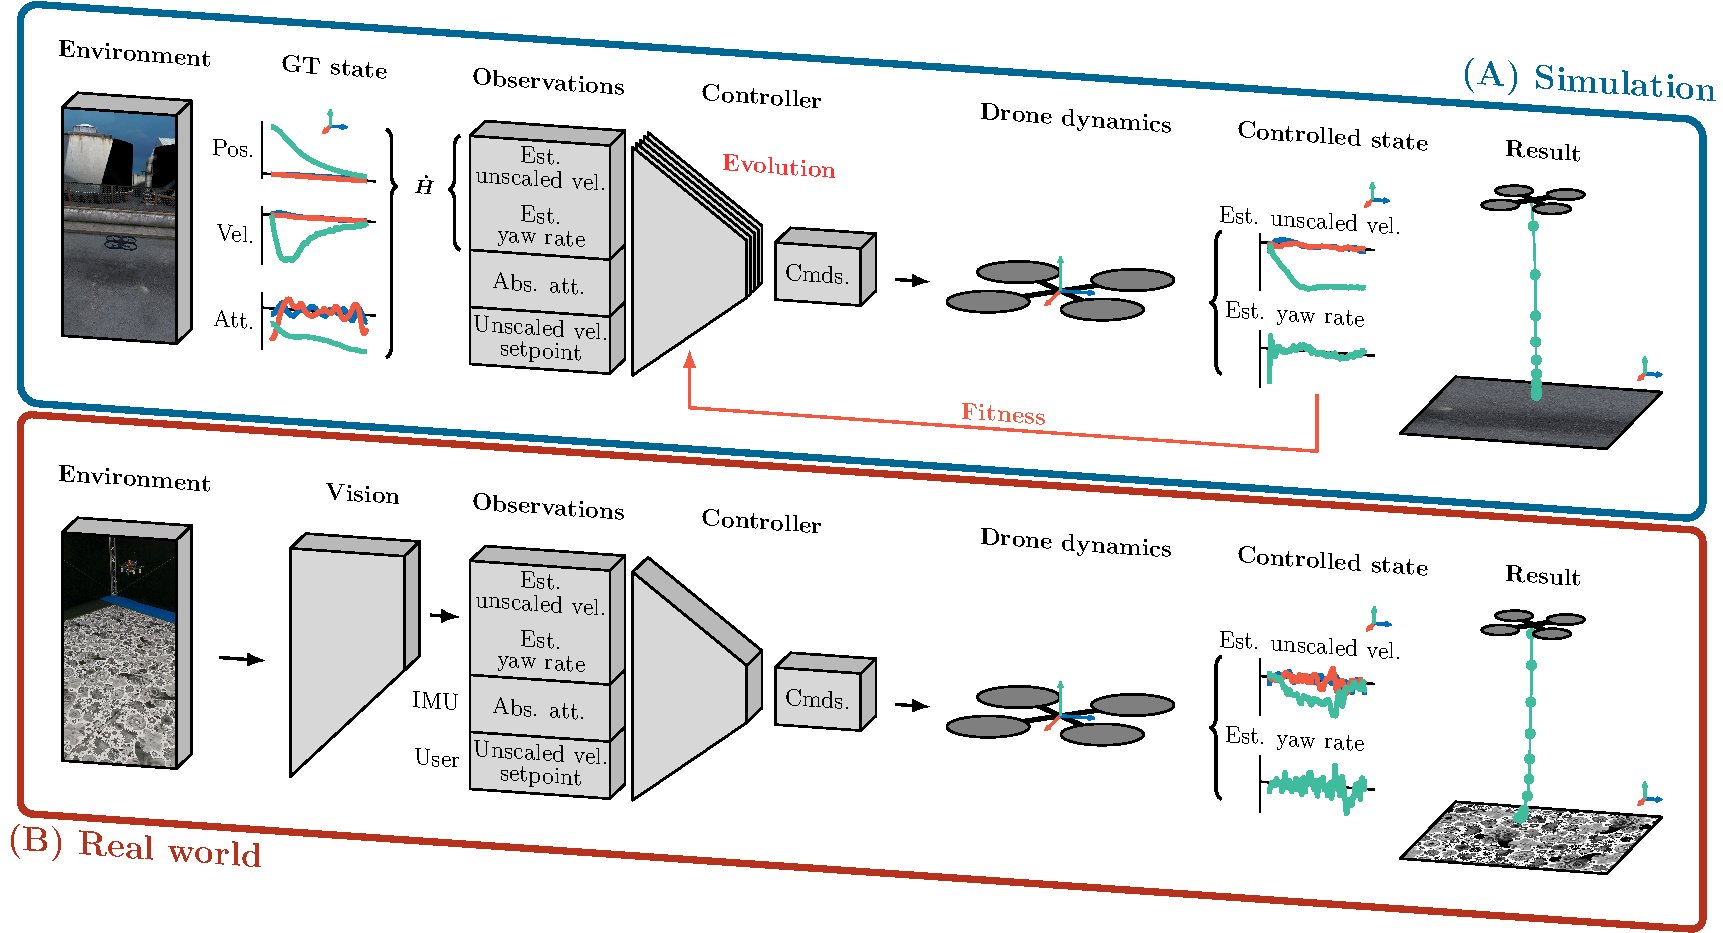
\includegraphics[width=0.975\textwidth]{04_chapters/SR23/figures/fig3-control.pdf}
	\caption{Overview of the control pipeline for simulation and real-world tests. During training in simulation, we construct visual observables (scaled velocities and yaw rate) from ground-truth using the continuous homography transform. The control decoding takes these observables together with roll and pitch and a setpoint to output commands, which control the drone dynamics. We train the controller using evolution based on a fitness signal that quantifies how well the controller can follow setpoints for horizontal and vertical flight. In the real world, we receive flows of the corner ROIs from the vision network, transform these to control commands in a single matrix multiplication, and send these commands to the autopilot.}
	\label{fig:sr_control}
\end{figure*}

\section{Method}

Here, we explain the main components of the proposed fully neuromorphic vision-to-control pipeline, starting with the neuron model of our SNN and how this is trained in a self-supervised fashion using real event camera data. Next, we describe how the vision-based state estimate can be used for navigation, and how we train a controller on top of it. Finally, we discuss the real-world tests and hardware and the performed energy benchmarks.

\subsection{Simulating the on-chip spiking neuron model}

In this study, we utilize a spiking neuron model based on the current-based leaky-integrate-and-fire (CUBA-LIF) neuron, whose membrane potential $U$ and synaptic input current $I$ at timestep $t$ can be written as:
\begin{align}
    U^{t}_{i} &= \tau_U (1 - S^{t-1}_{i}) U^{t-1}_{i} + I^{t}_{i} \\
    I^{t}_{i} &= \tau_I I^{t-1}_{i} + \sum_j w_{ij}^{\text{ff}} S_j^{t} + w_{ii}^{\text{rec}} S_i^{t-1}
\end{align}
where $j$ and $i$ denote presynaptic (input) and postsynaptic (output) neurons within a layer, $S \in \{0, 1\}$ a neuron spike, and $w^{\text{ff}}$ and $w^{\text{rec}}$ feedforward and self-recurrent connections (if any), respectively. The decays (or leaks) of the two internal state variables of this neuron model are learned, and are denoted by $\tau_U$ and $\tau_I$. A neuron fires an output spike if the membrane potential exceeds a threshold $\theta$, which is also learned. The firing of a spike triggers a hard reset of the membrane potential. Note that, in this work, all neurons within a layer share the same decays and firing threshold.

Neurons on the Loihi neuromorphic processor also follow the CUBA-LIF model \cite{davies2018loihi}, however, several considerations must be taken into account to accurately simulate these on-chip neurons. Firstly, the two states variables are quantized in the integer domain. Hence, the parameters associated with these variables are also quantized in the same way: $w\in[-256\ ..\ 256 - \Delta w]$ with $\Delta w$ being the quantization step for the synaptic weights, $\tau_{\{U,I\}}\in[0\ ..\ 4096]$ for the decays, and $\theta\in[0\ ..\ 131071]$ for the threshold. We follow this quantization scheme with $\Delta w=8$ (6-bit weights) in the simulation and training of our neural networks. Secondly, to emulate the arithmetic left (bit) shift operations carried out by the processor when updating the neuron states, we perform a rounding towards zero operation after the application of the decays. Taking these aspects into consideration, we obtain a matching score of 100\% between the simulated and the on-chip spiking neurons. We use quantization-aware training (quantized forward pass, floating-point backward pass) to minimize the performance loss of our SNN when deployed on Loihi.

As surrogate gradient for the spiking function $\sigma$, we opt for the derivative of the inverse tangent~\cite{fang2021incorporating}:
\begin{align}
    \sigma'(x) &= \text{aTan}' = 1/(1 + \gamma x^2) \\
    x &= u - \theta
\end{align}
with $\gamma=10$ being the surrogate width.

\subsection{Four-point parametrization to estimate homography}

Assuming that $\tilde{\boldsymbol{x}}=\left[\boldsymbol{x}^T, 1\right]^T$ and $\tilde{\boldsymbol{x}}'=\left[\boldsymbol{x}'\,^T, 1\right]^T$ are two undistorted corresponding points from a planar scene with pixel array coordinates $\boldsymbol{x}= [x,y]^T$ and $\boldsymbol{x}'= [x',y']^T$ expressed in homogeneous coordinates and captured by a pinhole camera at different time instances, a planar homography transformation is a linear projective transformation that maps $\tilde{\boldsymbol{x}}\leftrightarrow\tilde{\boldsymbol{x}}'$ such that:
\begin{align}\label{eq:homo}
    \lambda 
    \begin{bmatrix}
    x'\\
    y'\\
    1
    \end{bmatrix}
    =
    \boldsymbol{H}
    \begin{bmatrix}
    x\\
    y\\
    1
    \end{bmatrix};\quad \text{with } \boldsymbol{H}=
    \begin{bmatrix}
    h_{11} & h_{12} & h_{13}\\
    h_{21} & h_{22} & h_{23}\\
    h_{31} & h_{32} & h_{33}
    \end{bmatrix}
\end{align}
where $\boldsymbol{H}$ is a 3x3 non-singular matrix, further referred to as the homography matrix, which is characterized by eight degrees of freedom and is defined up to a scale factor $\lambda$, and from which we obtain the normalized form by setting $h_{33}=1$. 

From \eqnref{eq:sr_homo}, we can formulate a system of linear equations for the $k$-th point correspondence:
\begin{align}
    \boldsymbol{A}_k \boldsymbol{h} &= \boldsymbol{b}_k \\
    \boldsymbol{A}_k &=  
    \begin{bmatrix}
    x & y & 1 & 0 & 0 & 0 & -x'x & -x'y \\
    0 & 0 & 0 & x & y & 1 & -y'x & -y'y\\
    \end{bmatrix}\label{eq:4}\\
    \boldsymbol{h} &= 
    \begin{bmatrix}
    h_{11} & h_{12} & h_{13} & h_{21} & h_{22} & h_{23} & h_{31} & h_{32}
    \end{bmatrix}^T\\
    \boldsymbol{b}_k &=
    \begin{bmatrix}
    x' & y'
    \end{bmatrix}^T\label{eq:6}
\end{align}
As shown in \figref{fig:vision}A, our vision network predicts the displacement of the corner ROI pixels in a certain time window. Using this information, we can solve for the components of the homography matrix through:
\begin{equation}
    \boldsymbol{h}=\boldsymbol{A}^{-1}\boldsymbol{b}
\end{equation}
with $\boldsymbol{A}$ and $\boldsymbol{b}$ being the result of the concatenation of the individual $\boldsymbol{A}_k$ and $\boldsymbol{b}_k$ of each point correspondence $\forall\, k\in\{\mathrm{TL},\mathrm{TR},\mathrm{BR},\mathrm{BL}\}$, resulting in a determined system of equations. This approach is referred to as the four-point parametrization of the homography transformation \cite{baker2006parameterizing}, and it has proved to be successful in the event-camera literature for robotics applications \cite{sanket2020evdodgeneta, ozawa2022accuracya}.

Once the homography matrix is estimated, we can estimate a dense (per-pixel) optical flow map as follows:
\begin{align}\label{eq:flow}
    \boldsymbol{u}(\boldsymbol{x}, \boldsymbol{H})=
    \begin{bmatrix}
    u(\boldsymbol{x}, \boldsymbol{H})\\
    v(\boldsymbol{x}, \boldsymbol{H})
    \end{bmatrix}
    =
    \left(\boldsymbol{H}
    \begin{bmatrix}
    x\\
    y\\
    1
    \end{bmatrix}
    \right)_\mathrm{Eucl}
    - 
    \begin{bmatrix}
    x\\
    y
    \end{bmatrix}
\end{align}
which encodes the displacement of pixel $\boldsymbol{x}$ in the time window of $\boldsymbol{H}$. $(\cdot)_\mathrm{Eucl}$ indicates the conversion from homogeneous to Euclidean coordinates.

\subsection{Self-supervised learning of event-based optical flow}

To train our spiking architecture to estimate the displacement of the pixels of the four corner ROIs in a self-supervised fashion, we use the contrast maximization framework for motion compensation \cite{gallego2018unifying, gallego2019focusa}. Assuming constant illumination, accurate optical flow information is encoded in the spatiotemporal misalignments among the events triggered by a moving edge (blur). To retrieve it, one has to learn to compensate for this motion (deblur the event partition) by transporting the events through space and time. Once we get a per-pixel optical flow estimate $\boldsymbol{u}(\boldsymbol{x}, \boldsymbol{H})$ from \eqnref{eq:flow}, we can propagate the events to a reference time $t_{\text{ref}}$ through the following linear motion model:
\begin{equation}\label{eqn:motionmodel}
    \boldsymbol{x}'_i=\boldsymbol{x}_i + (t_{\text{ref}} - t_i)\boldsymbol{
    u}(\boldsymbol{x}_i, \boldsymbol{H})
\end{equation}
where $t$ and $t_\text{ref}$ are normalized relative to the time window between $\boldsymbol{x}$ and $\boldsymbol{x}'$. The result of aggregating the propagated events is the image of warped events (IWE) at $t_{\text{ref}}$, and it having a high contrast indicates good motion compensation/deblurring. 

As loss function, we use the reformulation from \cite{hagenaars2021selfsupervised} of the focus objective function based on the per-pixel and per-polarity average timestamp of the IWE \cite{mitrokhin2018eventbased, zhu2019unsuperviseda}. The lower this metric, the better the event deblurring and hence the more accurate the estimated optical flow. We generate an image of the per-pixel average timestamp for each polarity $p'$ via bilinear interpolation:
\begin{align}\label{eqn:timeimage}
    \begin{aligned}
        T_{p'}(\boldsymbol{x}{;}\boldsymbol{u} |t_{\text{ref}}) &= \frac{\sum_{j} \kappa(x - x'_{j})\kappa(y - y'_{j})t_{j}}{\sum_{j} \kappa(x - x'_{j})\kappa(y - y'_{j})+\epsilon}\\\kappa(a) &= \max(0, 1-|a|)\\
        j = \{i \mid p_{i}=&\ p'\}, \hspace{15pt}p'\in\{+,-\}, \hspace{15pt} \epsilon\approx 0
    \end{aligned}
\end{align}

Following \cite{hagenaars2021selfsupervised}, we first scale the sum of the squared temporal images resulting from the warping process with the number of pixels with at least one warped event:
\begin{equation}\label{eq:scaling}
    \mathcal{L}_{\text{contrast}}(t_{\text{ref}}) = \frac{\sum_{\boldsymbol{x}} T_{+}(\boldsymbol{x}{;}\boldsymbol{u} |t_{\text{ref}})^2 + T_{-}(\boldsymbol{x}{;}\boldsymbol{u} |t_{\text{ref}})^2}{\sum_{\boldsymbol{x}}\left[n(\boldsymbol{x}') > 0\right] + \epsilon}
\end{equation}
where $n(\boldsymbol{x}')$ denotes a per-pixel event count of the IWE.

As in \cite{zhu2019unsuperviseda, paredes-valles2021back, hagenaars2021selfsupervised}, we perform the warping process both in a forward ($t_{\text{ref}}^{\text{fw}}$) and in a backward fashion ($t_{\text{ref}}^{\text{bw}}$) to prevent temporal scaling issues during backpropagation. The total loss used to train our event-based optical flow networks is then given by:
\begin{align}\label{eq:flow_loss}
\mathcal{L}_{\text{contrast}} &= \mathcal{L}_{\text{contrast}}(t_{\text{ref}}^{\text{fw}}) + \mathcal{L}_{\text{contrast}}(t_{\text{ref}}^{\text{bw}})\\
\mathcal{L}_{\text{flow}} &= \mathcal{L}_{\text{contrast}} + \lambda_{\mathcal{L}} \mathcal{L}_{\text{smooth}}\label{eq:final_loss}
\end{align}
where $\mathcal{L}_{\text{smooth}}$ is a Charbonnier smoothness prior \cite{charbonnier1994two} applied in the temporal domain to subsequent per-corner-ROI optical flow estimates, while $\lambda_{\mathcal{L}}$ is a scalar balancing the effect of the two losses. We empirically set this weight to $\lambda_{\mathcal{L}}=0.1$.

As discussed in \cite{hagenaars2021selfsupervised, paredes2023taming}, there has to be enough linear blur in the accumulated input event partition for this loss function to be a robust supervisory signal \cite{gallego2019focusa, stoffregen2019eventa}. Since we process the event stream sequentially, with only a few events being considered at each forward pass, we define the so-called training partition:
\begin{equation}
    \boldsymbol{\varepsilon}^{\text{train}}_{k\rightarrow k+K}\doteq\{(\boldsymbol{\varepsilon}^{\text{inp}}_{i}, \boldsymbol{u}_i)\}_{i=k}^{K}
\end{equation}
which is a buffer that gets populated every forward pass with the input events and their corresponding optical flow estimates. This is illustrated in \figref{fig:vision}A. At training time, we perform a backward pass with the content of the buffer using backpropagation through time once it contains five successive event-flow tuples (25 milliseconds of event data), after which we update the model parameters, detach its states from the computational graph, and clear the buffer. Note that the selection of input and training partition lengths represents deliberate design choices~\cite{valerdi2023insights}, made in alignment with our target execution frequency of 200 Hz, the fact that we do not have direct connectivity between the event camera and the neuromorphic processor, and the statistical attributes of our dataset. We use a batch size of 16 and train until convergence with the Adam optimizer \cite{kingma2017adam} and a learning rate of $1\mathrm{e}{}$-$4$. We validate the quality of the estimated optical flow against the ground-truth optical flow using the average endpoint error (EPE) metric, which is defined as the Euclidean distance between predicted and ground-truth flow values averaged over all pixels in the image:
\begin{equation}
    \mathrm{EPE} = \frac{1}{N}\sum_{i\,\in\,I}^N \lVert \boldsymbol{u}_i - \boldsymbol{u}_i^\mathrm{GT} \rVert
\end{equation}
where $I$ is the set of $N$ pixels in the image, and $u^\mathrm{GT}$ is the ground-truth flow.

\subsection{From a vision-based state estimate to control}

The corner ROI flows $\left[\boldsymbol{u}_\mathrm{TL}^T,\boldsymbol{u}_\mathrm{TR}^T,\boldsymbol{u}_\mathrm{BR}^T,\boldsymbol{u}_\mathrm{BL}^T\right]^T \in \mathbb{R}^{8\times 1}$ resulting from the vision-based state estimation can be used to control the drone. More specifically, we can transform the flows to visual observable estimates~\cite{decroon2013opticflow}, consisting of unscaled velocities $\boldsymbol{\hat{\nu}}^\mathcal{C} \in \mathbb{R}^{3\times 1}$ and yaw rate $\hat{\omega}^\mathcal{C}_z$ in the camera frame $\mathcal{C}$, as follows~\cite{longuet-higgins1980interpretation}:
\begin{align}
    \boldsymbol{u} &=
    \begin{bmatrix}
        -1 & 0 & x & x \\
        0 & -1 & y & -y
    \end{bmatrix}
    \begin{bmatrix}
        \boldsymbol{\nu}^\mathcal{C}\\
        \omega_z^\mathcal{C}
    \end{bmatrix}
    \label{eq:visobs}
\end{align}
where $\boldsymbol{u}$ is the optical flow of a world point with pixel array coordinate $\boldsymbol{x} = [x,y]^T$, and where it is assumed that the scene is static and planar, angles in pitch and roll are small and optical flow is derotated in pitch and roll (meaning the observed flow is only due to translation and yawing). Concatenating \eqnref{eq:visobs} for all four corners of the field of view ($\boldsymbol{u}_k, \boldsymbol{x}_k\, \forall\, k\in\{\mathrm{TL},\mathrm{TR},\mathrm{BR},\mathrm{BL}\}$) allows us to do a least-squares estimation of the unscaled velocities $\boldsymbol{\hat{\nu}}^\mathcal{C}$ and the yaw rate $\hat{\omega}^\mathcal{C}_z$, which can then be transformed to the body frame $\mathcal{B}$. To perform control, we can let a user select visual observable setpoints $\boldsymbol{\nu}_{\mathrm{sp}}^\mathcal{B}$ and $\omega_{z,\mathrm{sp}}^\mathcal{B}$, and use a trained or manually tuned controller to minimize the difference between the estimated visual observables and their setpoints.

\begin{figure}[!t]
	\centering
	\includegraphics[width=\linewidth]{04_chapters/SR23/figures/fig7-merging.pdf}
%	\includegraphics[trim=40 400 0 0, clip, width=0.54\linewidth]{04_chapters/SR23/pdf/fig7-merging.png}
%	\includegraphics[trim=100 0 100 400, clip, width=0.425\linewidth]{04_chapters/SR23/pdf/fig7-merging.png}
	\caption{Merging linear transformations. (\textit{A}) We go directly from output spikes $\boldsymbol{s}$ of the vision network to control commands $\boldsymbol{c}$ in a single linear decoding by multiplying the involved linear transformation matrices. (\textit{B}) The same principle can be applied to connect two separately trained spiking networks in a spiking manner, from spikes $\boldsymbol{s}$ to currents $\boldsymbol{c}$, suitable for neuromorphic hardware.}
	\label{fig:sr_merge}
\end{figure}

Because \eqnref{eq:sr_visobs} is a linear transformation, it can be ``merged'' with other transformations if these are also linear. This holds for the decoding from spikes to corner ROI flows in the vision SNN, meaning that we can use a single linear transformation from spikes to control commands if we use a linear controller. In a similar fashion, we can use this idea to connect separately trained SNNs, merging their linear decodings and encodings. If both are implemented on neuromorphic hardware, this would mean that no off-chip transfer is necessary. \figref{fig:sr_merge} illustrates these concepts.

\subsection{Training control in simulation}

We perform control by linearly transforming the visual observable estimates $\boldsymbol{\hat\nu}^\mathcal{B} \in \mathbb{R}^{3\times 1}$ and $\hat\omega_z^\mathcal{B}$, the drone's absolute roll $\lvert\phi\rvert$ and pitch $\lvert\theta\rvert$ and the unscaled velocity setpoint $\boldsymbol{\nu}^\mathcal{B}_{\mathrm{sp}} \in \mathbb{R}^{3\times1}$ to a control command $\boldsymbol{c} \in \mathbb{R}^{4\times 1}$, which consists of an upward, mass-normalized collective thrust offset from hover $\bar{f}_{0,c}$ in the body frame $\mathcal{B}$, a roll angle $\phi_c$ and pitch angle $\theta_c$, and a yaw rate $\omega^\mathcal{B}_{z,c}$, in order to reach a certain setpoint of unscaled velocities $\boldsymbol{\nu}_{\mathrm{sp}}^\mathcal{B}$ and yaw rate $\omega_{z,\mathrm{sp}}^\mathcal{B}$ (always 0).

The control part is trained separately from the vision part because of the cost of accurately simulating event-based camera inputs (this needs subpixel displacements between frames, hence high frame rate for fast motion). Simulation is done with a modified version of the drone simulator Flightmare \cite{song2020flightmare}. To mimic the output of the vision-based state estimation network, we first compute the ground-truth continuous homography \cite{ma2004invitation,zhong2020direct} from the state of the drone:
\begin{align}
    \boldsymbol{\dot{H}} &= \boldsymbol{K} \left( [\boldsymbol{\omega}^\mathcal{C}]_\times + \frac{1}{p^\mathcal{WC}_z}\boldsymbol{v}^\mathcal{C}(\boldsymbol{e}^\mathcal{W}_{-z})^T \right) \boldsymbol{K}^{-1}
\end{align}
where $\boldsymbol{\dot{H}}$ is the continuous homography, $\boldsymbol{K}$ is the camera intrinsic matrix, $[\boldsymbol{\omega}^\mathcal{C}]_\times \in \mathbb{R}^{3\times 3}$ is a skew-symmetric matrix representing infinitesimal rotations, $p_z^\mathcal{WC}$ is the Z-component of the position vector from the world frame $\mathcal{W}$ to the camera frame $\mathcal{C}$ (representing perpendicular distance from the ground plane to the camera), $\boldsymbol{v}^\mathcal{C}$ is the velocity of the camera, and $\boldsymbol{e}_{-z}^\mathcal{W}$ is the unit vector in the negative Z-direction of the world frame. To obtain angular rates and velocities in the camera frame, we use the camera extrinsics, consisting of a rotation $\boldsymbol{R}^\mathcal{CB}$ and a translation $\boldsymbol{T}^\mathcal{CB}$:
\begin{align}
    \boldsymbol{\omega}^\mathcal{C} &= \boldsymbol{R}^\mathcal{CB} \boldsymbol{\omega}^\mathcal{B}\label{eq:wc} \\
    \boldsymbol{v}^\mathcal{C} &= \boldsymbol{R}^\mathcal{CB} \left( \boldsymbol{v}^\mathcal{B} + [\boldsymbol{\omega}^\mathcal{B}]_\times \boldsymbol{T}^\mathcal{CB} \right)\label{eq:vc}
\end{align}
where the right-hand sides of \eqnreftwo{eq:wc}{eq:vc} are known from the simulator. Next, we use the continuous homography to get the flow of the four corners~\cite{ma2004invitation,zhong2020direct}:
\begin{align}
    \boldsymbol{u}_k &= \left(-\left(\boldsymbol{1} - \tilde{\boldsymbol{x}}_k(\boldsymbol{e}^\mathcal{W}_{-z})^T\right)\boldsymbol{\dot{H}}\tilde{\boldsymbol{x}}_k\right)_\mathrm{Eucl}
\end{align}
where $\boldsymbol{u}_k$ is the flow in Euclidean coordinates, $\boldsymbol{1}$ is the identity matrix, and $\tilde{\boldsymbol{x}}_k = [x_k,y_k,1]^T$ is the projection of the world points in the corners of the field of view onto the pixel array in homogeneous coordinates (so, $\tilde{\boldsymbol{x}}_{\mathrm{BL}} = [0,180,1]^T$ and $\tilde{\boldsymbol{x}}_{\mathrm{TR}}=[180,0,1]^T$, note the difference with respect to \eqnref{eq:visobs}). We add $\mathcal{N}(0, 0.025)$ noise to the flows $\boldsymbol{u}_k$ (based on a characterization of the vision SNN). \eqnref{eq:visobs} is subsequently used to go from flows of the corner ROIs to visual observables in the camera frame, which is then transformed back to the body frame for control. Note that relating camera motion to the motion of points in the image (flow) can equivalently be done with the image Jacobian or feature sensitivity matrix~\cite{corke2011robotics}.

We use a mutation-only evolutionary algorithm with a population size of 100 to evolve the weights of the linear controller matrix $\in \mathbb{R}^{4\times 9}$, whose initial values are drawn from $\mathcal{U}(-0.1, 0.1)$. More specifically, we generate offspring by adding mutations drawn from $\mathcal{N}(0, 0.001)$ to all parameters of each parent and then evaluate the fitness of both parents and offspring. The next generation is comprised of the best 100 individuals, and we repeat this process until convergence (approx. 25k generations). We use Flightmare to assess fitness at flying various visual observable setpoints: every individual is evaluated across a set of 16 setpoints, with each unscaled velocity setpoint $\boldsymbol{\nu}^\mathcal{B}_{\mathrm{sp}}$ having at most one nonzero element $\in \{\pm0.2,\pm0.5,\pm1.0\}$~1/s, skipping the positive setpoints for the Z-direction, and including hover. The yaw rate setpoint is set to $\omega_{z,\mathrm{sp}}^\mathcal{B}=0$ for all. Each setpoint is repeated ten times, meaning a total of 160 evaluations per individual. Fitness $F$ is computed as:
\begin{align}
    F &= \frac{1}{N_\mathrm{eval}} \sum_{i \in N_\mathrm{eval}} \sum_{j \in N_{\mathrm{steps}}} \boldsymbol{w} \cdot \left( \boldsymbol{\nu}^\mathcal{B}_{\mathrm{sp},i} -
    \begin{bmatrix}
        \hat{\nu}_x^\mathcal{B}\\
        \hat{\nu}_y^\mathcal{B}\\
        \nu_z^\mathcal{W}
    \end{bmatrix}_j\,
    \right)^2 + \left(\hat{\omega}_z^\mathcal{B}\right)^2
\end{align}
Here, $N_{\mathrm{eval}}$ is the number of evaluations, $N_\mathrm{steps}=1000$ is the number of steps per evaluation, and $\boldsymbol{w}=[1, 1, w_z]^T$ is a vector weighing the fitness for different axes, where we set $w_z=10$ for setpoints where $\nu^\mathcal{B}_{z,\mathrm{sp}}=0$. Note that, for the Z-direction, we use the ground-truth unscaled velocity in the world frame $\nu_z^\mathcal{W}$ instead of the one in the body frame, as the latter is zero in the case of the drone ascending or descending at a slope equal to its attitude, and would hence go unpunished, leading to extra vertical drift. Furthermore, if the simulated drone goes out of bounds or crashes before the end of an evaluation, it will be reset without any additional fitness penalty.

We use domain randomization~\cite{tobin2017domain} to obtain a more robust controller and reduce the reality gap: for each of the ten repeats, a random constant bias $\mathcal{U}(-0.001, 0.001)$~rad is added to the absolute pitch and roll received by the control layer. This bias is shared among the population to keep things fair. Furthermore, for each of the 160 evaluations per individual, we randomly vary the initial position $\boldsymbol{p}^\mathcal{WB} = [0,0,2]^T + \mathcal{U}^{3\times1}(-1, 1)$ m (except for horizontal flight, where we fix $p^\mathcal{WB}_{z}$ to 1.5~m, due to the linear nature of the controller we have here, as explained later), initial velocity $\boldsymbol{v}^\mathcal{WB} \sim \mathcal{U}^{3\times1}(-0.02, 0.02)$~m/s, initial attitude quaternion $\boldsymbol{q}^\mathcal{WB} \sim \mathcal{U}^{4\times1}(-0.02, 0.02)$ (normalized), and initial angular rates $\boldsymbol{\omega}^\mathcal{B} \sim \mathcal{U}^{3\times1}(-0.02, 0.02)$~rad/s.

We modify Flightmare to include drag $\boldsymbol{f}_\mathrm{drag}$ occurring as a result of translational motion, and we take it to be acting in the so-called ``flat-body'' frame $\mathcal{B'}$, which is the body frame rotated by the roll and pitch of the drone, such that the Z-axis is aligned with the world Z-axis. Following~\cite{dewagter2022sensing}, we use a drag model that is linear with respect to velocity in X and Y, but using a drag coefficient $k_{v,x}=k_{v,y}=0.5$. This results in the following:
\begin{align}
    \boldsymbol{f}_\mathrm{drag}^\mathcal{B} &= -\boldsymbol{R}^\mathcal{BB'}
    \left(
    \begin{bmatrix}
        k_{v,x} \\
        k_{v,y} \\
        0
    \end{bmatrix}
    \circ \boldsymbol{R}^\mathcal{B'B}\boldsymbol{v}^\mathcal{B}
    \right)
\end{align}

The outputs of the linear controller $\boldsymbol{c}\in \mathbb{R}^{4\times1}$ are clamped to $[-1,1]$ and fed to different parts of the cascaded low-level (thrust, attitude and rate) controllers. To accommodate some of the shortcomings of the linear controller, we compensate thrust for the attitude of the drone.

All dynamics equations are integrated with 4$^{\mathrm{th}}$-order Runge-Kutta with a timestep of 2.5~ms. The frequency of the simulation is 50~Hz. %All remaining details can be found in the Supplementary Methods.

% \subsection{From simulation to the real world}

% We achieve successful sim-to-real transfer through several strategies. One is domain randomization~\cite{tobin2017domain}, which we do by adding noise to the observed flows, through a random bias on the attitude estimate, and by varying the initial conditions of the simulated quadrotor. Another is abstraction~\cite{scheper2017abstraction}, which we do by making use of low-level controllers to go from thrust and attitude to rotor speeds and by calibrating the attitude and hover thrust biases before each flight to make sure they are small/zero (as in the simulator). Finally, we smooth (low-pass filter) and scale the computed visual observables and tune the gains scaling the control layer outputs in the real world.

% \eqnref{eq:visobs} is used to transform the flows of the corner ROIs coming from the vision network into visual observables (unscaled velocities $\boldsymbol{\hat{\nu}}^\mathcal{B}$ and yaw rate $\hat{\omega}^\mathcal{B}_z$), absolute roll $\lvert\phi\rvert$ and pitch $\lvert\theta\rvert$ are taken from the drone's accelerometers, and the unscaled velocity setpoint $\boldsymbol{\nu}^\mathcal{B}_{\mathrm{sp}}$ is provided by the user. The yaw rate setpoint $\omega_{z,\mathrm{sp}}^\mathcal{B}=0$ is fixed.

% Extra experiments were performed by connecting the vision network to a hand-tuned proportional-integral (PI) controller. All remaining details can be found in the Supplementary Methods.

\subsection{Hardware setup}

Real-world experiments were performed with a custom-built quadrotor carrying the event-based camera (DVS 240), a single-board computer (UP Squared) and a neuromorphic processor (Intel Kapoho Bay with two Loihi neuromorphic research chips). A high-level overview can be found in \figref{fig:pipeline}, with all components are listed in \tabref{tab:components}. We use PX4 as autopilot firmware, and ROS (Robot Operating System) for communication. More specifically, events coming from the event-based camera are passed to the UP Squared over USB (Universal Serial Bus) using ROS1. These events are processed (downsampling, cropping, limiting to 90 per image corner ROI) on the UP Squared, and sent as spikes to the vision network running on the Kapoho Bay over USB. After processing, the output spikes are sent back over USB to the UP Squared, where they are decoded into flows for each corner ROI. The ROI flows are then published by a ROS1 node, and sent to ROS2 over a ROS1-ROS2 bridge. The linear controller (or PI controller, for that matter) and the processing around it, running as a ROS2 node, takes the ROI flows together with the attitude estimate coming from PX4 (IMU) and the ego-motion setpoint provided by the user, and outputs the control command. This command is then sent over ROS2 to PX4, and processed by the low-level controllers there. ROS2 makes use of RTPS (real-time publish-subscribe) for communication, which allows for high-frequency and high-bandwidth messaging between the UP and PX4, meaning our entire pipeline can run at 200~Hz\textemdash approximately the frequency of PX4's attitude controller. This attitude control frequency was a major driver for our choice to run the neuromorphic pipeline at the same frequency. This choice also depended on various other factors, ranging from the trade-off between a fast execution frequency and good optical flow estimation to the limitations of the spike interfacing over USB. Importantly, a 5~ms event window turned out to give accurate optical flow estimates, as well as a very fast execution frequency (see Supplementary Methods). Moreover, this frequency can be attained reliably, as Table \ref{tab:energy} shows that Intel's Loihi inference time is consistently faster than 5~ms. For position control between test runs, and as failsafe, we use an OptiTrack motion capture system.

% We estimate power required for hover flight by flying with a fully charged battery until a certain voltage, keeping track of time, and estimating spent mAh using the value from the charger. During this flight, the UP Squared is powered on (needed for control), and we estimate a power consumption of 277~W. Subtracting the estimated 18~W for the UP Squared makes the 259~W for the remaining components in \tabref{tab:components}. For the Kapoho Bay, we use the numbers from the performed energy benchmark, given that running power is almost equal to idle power. We get power estimates for the UP Squared (version UPS-APLX7-A20-0864) and DVS 240 from online available datasheets.

\begin{table}[!t]
	\centering
	\resizebox{0.85\linewidth}{!}{%
	\begin{tabular}{@{}llrr@{}}
		\thickhline
		\thickhline
		Component     & Product & Mass [g] & $\sim$Power [W]               \\ \midrule
		Frame                  & GEPRC Mark 4 225~mm &  \multirow{5}{*}{508} & \multirow{5}{*}{259}           \\
		Motor                  & Emax 2306 Eco II Series & &        \\
		Propellor              & Ethix S5 5~inch  & &               \\
		Flight Controller      & Pixhawk 4 Mini  &   &              \\
		ESC                    & SpeedyBee 45A BL32 4in1  &     &   \\ \midrule
		Battery                & Tattu FunFly 1800mAh 4S  & 195   &  -  \\ \midrule
		Single-board computer  & UP Squared ATOM Quad Core 08/64  & 202 & 18 \\ \midrule
		Event-based camera           & DVS 240  & 27     &      1\\ \midrule
		Neuromorphic processor & Intel Loihi, Kapoho Bay form factor  &  62   &   1\\ 
		\thickhline
		\thickhline
	\end{tabular}}
	\caption{List of hardware components used for the real-world test flights.}
	\label{tab:sr_components}
\end{table}

\subsection*{Energy benchmark}

Energy benchmarks for Loihi were performed on a Nahuku board (host machine: Intel Xeon Platinum 8280 CPU at 2.7 GHz, 126 GB RAM, Ubuntu 20.04, NxSDK 1.0.0), which contains 32 Loihi chips, as Kapoho Bay does not support energy probing. These (software) probes report a variety of power measurements, as well as execution times. Following the documentation, static power is due to transistor leakage, dynamic power is due to switching, idle power is measured while the embedded CPU cores on Loihi are still clocked but the neuromorphic are inactive, and total/running power is due to all components together. Kapoho Bay does support probing execution times, which we used to confirm that these are almost identical between Nahuku and Kapoho Bay. Furthermore, documentation states that Nahuku shuts down unused chips, meaning it can emulate energy consumption of a Kapoho Bay (which has two chips) with minimal overhead. Still, these benchmarks are not very representative of actual use on a drone, because that involves receiving and processing streaming data in an online fashion, whereas here all data is loaded to memory beforehand, and then processed as quickly as possible. Therefore, what these benchmarks represent is not the energy consumption and execution speed of the whole pipeline, but rather that of the network alone, without any bottlenecks and influences due to I/O and preprocessing. This also explains the much higher execution frequencies of Loihi with respect to real world tests, where this was always around 200~inf/s.

On Jetson Nano, we simulate the SNN and ANN in PyTorch (ARM Cortex-A57 CPU at 1.43 GHz, 4 GB RAM, Ubuntu 20.04, PyTorch 1.12.0). Jetson Nano has two power modes: a low-power (5W) mode, and a max-power (10W) mode, the difference being the number of active CPU cores (two versus four) and the frequencies of the active CPU and GPU cores. Power consumption was measured using the tegrastats utility, and execution time was measured in Python code. Note that the split between static and dynamic power cannot be made here as these are not available as measurements. Idle power is measured for a period of time after running the benchmarks.

\subsection*{Statistical analysis}

Unless mentioned otherwise, figures and tables show individual runs without any statistical method applied. Reported EPEs (as in \tabref{tab:AEEchanges}) are averaged over sequences in the test dataset. Reported drifts (as in Tables \ref{tab:simsnndrifts}, \ref{tab:realsnndrifts} and \ref{tab:realpidrifts}) are averaged over all runs in a certain flying direction.

For investigating the influence of the tether on the drone dynamics (see Supplementary Results), we performed a Z-test with sampling distributions created using bootstrapping~\cite{cohen1995empirical} and a confidence interval of 95$\%$ was used to determine significance.

\section{Experiments}

Because of the split between the vision and control parts of the pipeline, we can evaluate their performance separately. The estimated corner ROI flows of the vision part are compared against ground truth data obtained from a motion capture system, while the control part is evaluated in simulation. Connecting vision and control together, we then demonstrate the performance of our fully neuromorphic vision-to-control pipeline through real-world flight tests. To further illustrate the robustness of our vision-based state estimation, we perform real-world tests with changing setpoints, and tests in various lighting conditions. Lastly, we compare energy consumption against possible on-board GPU solutions.

\begin{figure*}[!h]
	\centering
	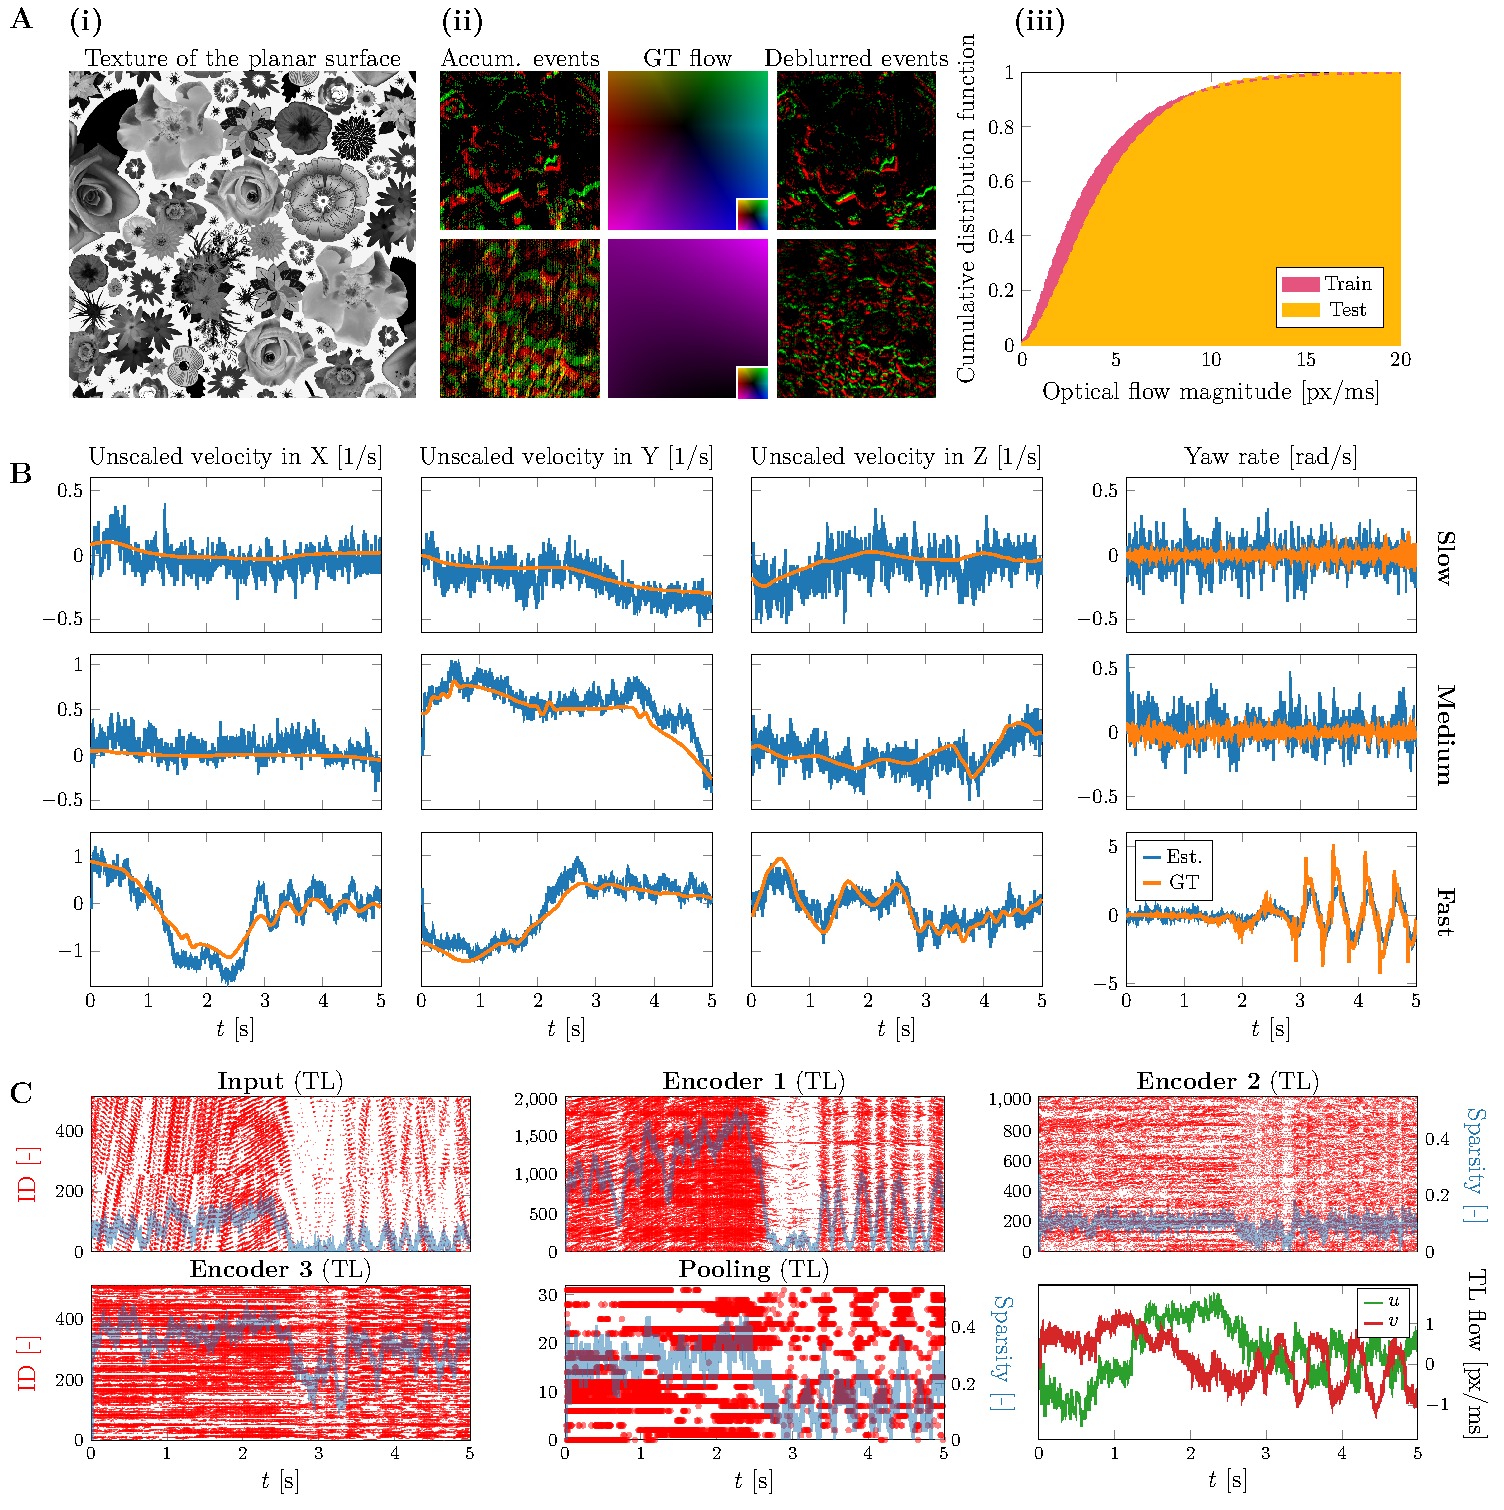
\includegraphics[width=\textwidth]{04_chapters/SR23/figures/fig4-vision-results.pdf}
	\caption{Overview of results for the vision-based state estimation. (\textit{A}) Characteristics of the dataset for estimating planar optical flow. \emph{Left:} Grayscale flower texture used to cover the floor. \emph{Center:} Accumulated event windows showing the blur arising from motion, ground truth flow fields as determined with a motion tracking system and based on a flat floor assumption (only for evaluation), and the result when using the flow fields to deblur the event windows (only for illustration). \emph{Right:} Ground-truth optical flow distributions for the training and test datasets. (\textit{B}) Comparison of estimated and ground-truth visual observables for sequences with different motion speeds (slow, medium, fast). (\textit{C}) Network activity resulting from the events in the top-left-corner ROI in the fast motion sequence.}
	\label{fig:sr_vision_results}
\end{figure*}

\subsection{Robust vision-based state estimation}

\begin{table*}[!t]
	\centering
	\resizebox{0.95\textwidth}{!}{%
		\begin{tabular}{@{}lrrrrr@{}}
			&&&&&\multicolumn{1}{r}{$\cdot 10^{-2}$}\\
			\thickhline
			\thickhline
			&  Full image   & +2x Down. & +Corner ROI crop & +Limit events & +Loihi quant. \\ \midrule
			Conv-GRU ANN                      & 5.88    & 5.56      & 5.61       & 5.72    & -       \\ \midrule
			Conv-RNN SNN                      & 7.92    & 7.89      & 7.91       & 6.97    & 6.96      \\ \midrule
			Self-RNN SNN (ours)                      & 10.79    & 9.80      & 8.22       & 7.71    & \textbf{8.34}      \\ 
			\thickhline
			\thickhline
		\end{tabular}
	}
	\caption{Quantitative comparison between different vision architectures. Bottom right corner, in bold, indicates the final architecture. Architecture choices (row-wise) and design decisions (column-wise) impact test performance in terms of the average endpoint error (EPE$\downarrow$, lower is better). Baseline architectures feature the same feedforward connectivity pattern as ours, but vary the neuron model and the type of recurrent connections.}
	\label{tab:sr_AEEchanges}
\end{table*}

To prevent reality-gap issues when simulating an event-based camera, we trained and evaluated the vision part of our pipeline using real-world event sequences recorded with the same platform (drone and downward-facing event-based camera) and in the same indoor environment (static and planar, constant illumination). This dataset consists of approximately 40 minutes of event data, which we split into 25 minutes for training and 15 for evaluation, and its motion distributions are shown in \figref{fig:vision_results}A. In addition to the visual data, the ground truth pose (position and attitude) of the drone over time was provided at a rate of 180 Hz, and was used solely for evaluation. Examples of this ground truth, which can be converted to dense optical flow using the camera calibration, are shown in \figref{fig:vision_results}A alongside the floor texture of the indoor environment. %Note that this dataset is available with the Supplementary Material of this work. Furthermore, to demonstrate that using the same texture for training and evaluation does not lead to overfitting (and resulting degraded control performance), we performed additional experiments with different types of texture that can be found in the Supplementary Material.

We trained our vision SNN with the self-supervised contrast maximization framework from \cite{hagenaars2021selfsupervised} and a quantization-aware training routine that simulates the neuron and synapse models in the target neuromorphic hardware. Afterwards, we evaluated the performance of our spiking network on the task of planar event-based optical flow estimation using sequences with varying amounts of motion. Qualitative results are presented in \figref{fig:vision_results}B, where the estimated visual observables (unscaled velocities and yaw rate, constructed from the estimated optical flow vectors at the image corner ROIs) are compared to their ground-truth counterparts. These results confirm the validity of our approach. Despite the architectural limitations of the proposed solution (for instance, lower resolution due to binary activations, limited field of view, only self-recurrency, weight and state quantization) and the fact that it does not have access to ground-truth information during training, it was able to produce optical flow estimates that accurately capture the motion encoded in the input event stream (the ego-motion of the camera), even for the fast rotation of approximately 4~rad/s at the end of the shown sequence. Note that, similarly to any other optical-flow-based state-estimation solution, our SNN is subject to the aperture problem not only due to the limited receptive field of the corner ROIs but also because of the use of event cameras as vision sensors \cite{gallego2020eventbased}.

In \figref{fig:vision_results}C, we show the internal spiking activity of our vision SNN as it processes the top-left corner ROI from the fast sequence shown in \figref{fig:vision_results}B, along with the decoded optical flow vectors. These qualitative results provide insight into the type of processing carried out by the proposed architecture, which is spike-based and therefore sparse and asynchronous. Notably, despite the rapid motion in the input sequence, all layers of the SNN maintained activation levels below 50\% of the available neurons. Note that the network was not explicitly trained to promote sparse activations, but could perhaps be rendered even more energy efficient by including sparsity measures in the loss function. Furthermore, we can distinguish layers with activity levels that are highly correlated with the input activity (encoder 1 and pooling), and layers that rely on their explicit recurrent connections to maintain activity levels that are relatively independent of the input statistics (encoder 2 and encoder 3). This observation could be the starting point for a future investigation into how this type of network determines optical flow (as in~\cite{dejong2021neural}).

In \tabref{tab:AEEchanges}, we provide a quantitative comparison of our solution with other similar recurrent architectures (that are not compatible or do not fit in the Intel Kapoho Bay), based on the average endpoint error (EPE, the Euclidean distance between predicted and ground-truth optical flow vectors averaged over all pixels in the image). This evaluation not only demonstrates the accuracy of our spiking network, but also assesses the effect of each mechanism that was incorporated into the pipeline to achieve a solution that could be deployed on Loihi at the target frequency of 200~Hz (downsampling the image space, only processing the events from the corner ROIs, limiting the maximum number of processed events per corner, and adding quantization; see also the Supplementary Methods). Several observations could be made. Firstly, the ANN outperformed its spiking variants by a large margin. This is likely due to the higher resolution of the floating point activations and the direct relation between the backpropagation gradient and the output error. Secondly, self-recurrency (Self-RNN) was the weakest form of explicit recurrency among those tested. The other networks seemed to successfully exploit their capability of representing more complex temporal functions.
Thirdly, deploying one architecture to each image corner ROI instead of processing the entire image space at once was beneficial for our architecture (lowering the EPE from 9.80 to 8.22), but had a slight detrimental effect on the baselines. This may be due to the dataset containing ample texture on the floor. A dataset with much less texture might have shown a different result. Fourthly, limiting the number of events that can be processed at once to 90 per corner ROI was also helpful for the evaluated SNNs, as it helped reduce the internal activity levels. Lastly, the incorporation of the Loihi-specific weight and state quantization led to an error increase for our architecture.

\begin{figure*}[!t]
	\centering
	\vspace{10pt}
	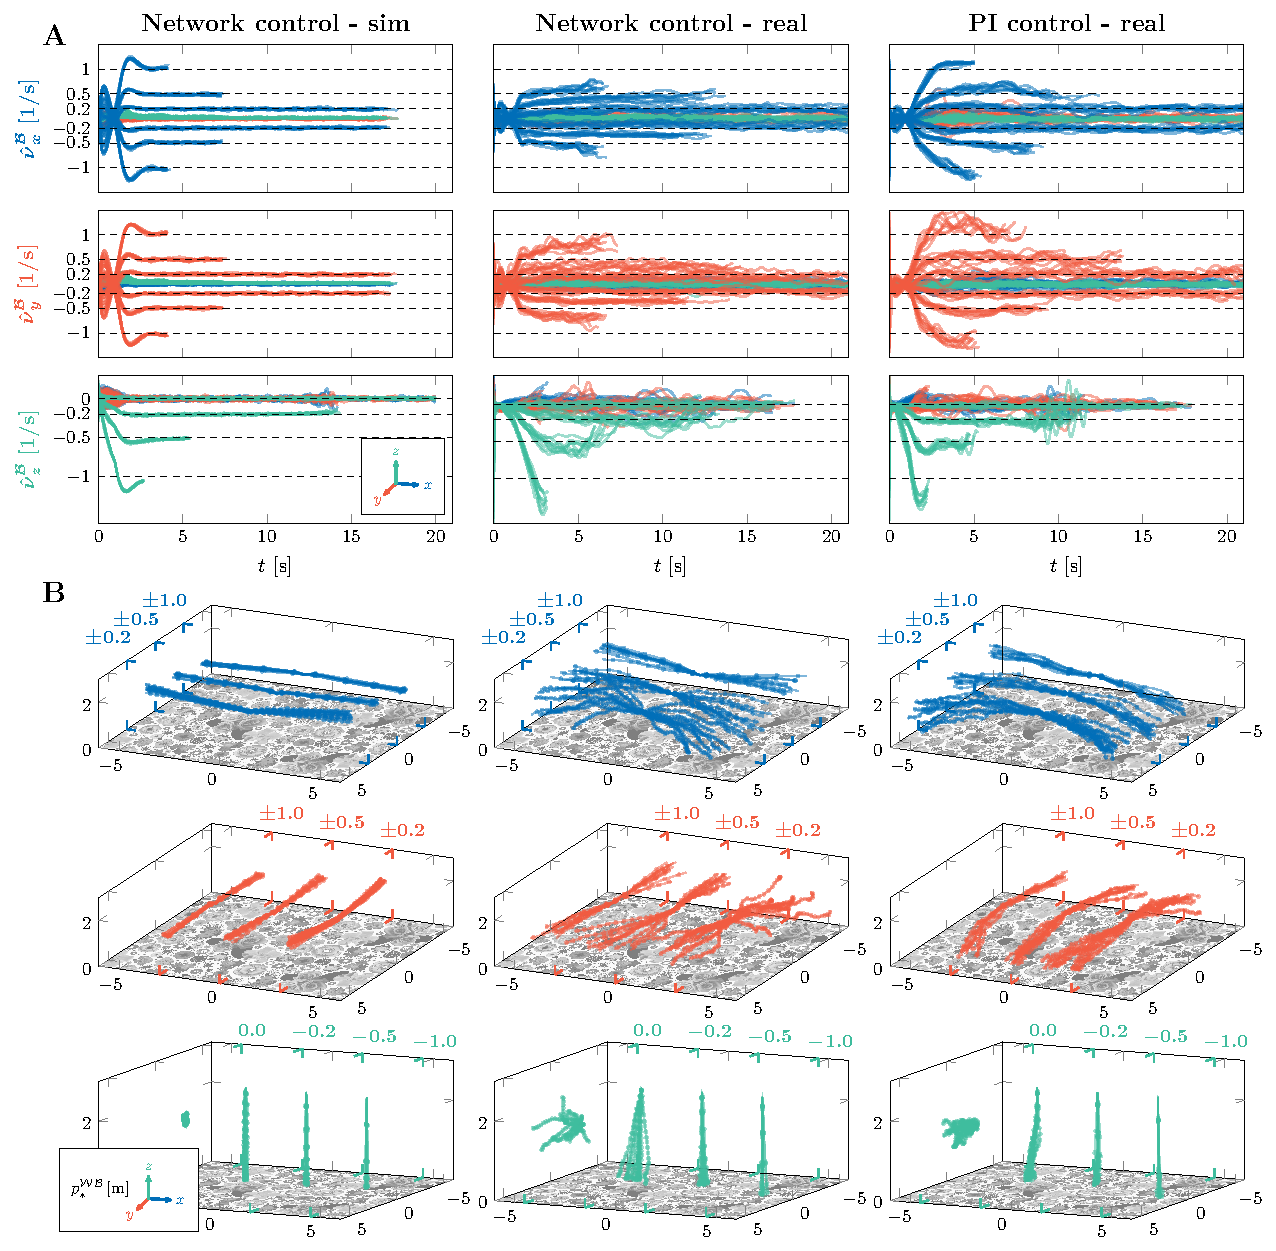
\includegraphics[width=\textwidth]{04_chapters/SR23/figures/fig5-simnetpi-results.pdf}
	\caption{Comparison of results obtained in simulation and during real-world flight tests. (\textit{A}) Estimated scaled velocities for 16 different setpoints in three axes, across three scenarios: linear network controller in simulation and the real world, and a hand-tuned proportional-integral (PI) controller in the real world. Real-world tests use the vision network to obtain visual observable estimates. Setpoints are nonzero in one direction, indicated with dashed lines. Rows represent the different motion axes. (\textit{B}) 3D world position trajectories for the same flight tests. Each cube in (\textit{B}) matches the plot in the corresponding location in (\textit{A}).}
	\label{fig:sr_results1}
\end{figure*}

\subsection{Control through visual observables: From sim to real}

Separately from the vision part, we trained and evaluated the control part of our pipeline. Due to limitations in the hardware setup (see Materials and Methods), this is a linear mapping from a visual observable estimate, absolute roll and pitch and a visual observable setpoint to thrust and attitude commands. The visual observable estimate is made up of unscaled velocity $\boldsymbol{\hat{\nu}}^\mathcal{B}$ and yaw rate $\hat{\omega}^\mathcal{B}_z$; the visual observable setpoint consists of the corresponding setpoints in unscaled velocity $\boldsymbol{\nu}^\mathcal{B}_{\mathrm{sp}}$ and yaw rate $\omega^\mathcal{B}_{z,\mathrm{sp}}$.
A population of these linear mappings was evolved in simulation for a set of 16 unscaled velocity and yaw rate setpoints. Each unscaled velocity setpoint $\boldsymbol{\nu}^\mathcal{B}_{\mathrm{sp}}$ had at most one nonzero element $\in \{\pm0.2,\pm0.5,\pm1.0\}$~1/s. In other words: they represented hover, vertical flight in the form of landing at three speeds (no ascending flight), and horizontal flight in four directions at three speeds. Unless mentioned otherwise, the setpoint for yaw rate $\omega^\mathcal{B}_{z,\mathrm{sp}} = 0$. \figref{fig:results1} shows the performance of the evolved linear network controller in simulation in terms of the estimated unscaled velocities $\boldsymbol{\hat{\nu}}^\mathcal{B}$ (\figref{fig:results1}A) and the world position $\boldsymbol{p}^\mathcal{WB}$ over time (\figref{fig:results1}B) for all setpoints. The control performance was satisfactory; The controller reached the setpoint in all cases, and was capable of keeping the unscaled velocities for the non-flight direction close to zero. Especially for $\nu_{*,\mathrm{sp}}^\mathcal{B}=\pm1.0$~1/s, some overshoot was witnessed, but this could be expected given that this is a linear mapping without any kind of derivative control.

\figref{fig:results1} furthermore shows the results obtained by deploying this controller in the real world, and replacing the ground-truth visual observables with those estimated by the vision network (also see Movie S3). Overall, the results demonstrated successful deployment of the fully neuromorphic vision-to-control pipeline. Looking at the unscaled velocity plots for the different setpoints, we see that these became less noisy for higher setpoints and faster flight, as can also be seen from the 3D position plots. This is due to the fact that the signal-to-noise ratio of the vision-based state estimation increased with motion magnitude (little motion means most events are due to noise, as can be seen in \figref{fig:vision_results}). Also, the inertia of the drone provided some stability at higher speeds. Nevertheless, apart from several setpoints (for example, landings, $\nu^\mathcal{B}_{\{x,y\},\mathrm{sp}} = \pm0.2$~1/s), the controller was not always able to reach the desired setpoint: the steady-state error looked to be proportional to the setpoint magnitude. This could be attributed to the fact that although the controller is a linear mapping, the relationship between attitude angle and resulting forward/sideways velocity is nonlinear (especially at larger attitude angles), and additionally affected by drag.
Providing absolute attitude input to the network, and simulating the drag (as in \cite{dewagter2022sensing}) during training turned out not to be enough to compensate, and small errors were accumulated over time. Furthermore, there can be mismatches between the dynamics of the simulated drone (body characteristics, motor dynamics) with which the controller was trained and the real drone on which the flight tests were performed, even though we abstracted the control outputs to attitude commands. Lastly, inaccuracies of the drag model can also be a source of error (in this case, it seems that drag was higher in reality than in simulation). A linear or proportional controller, such as we have here, cannot integrate all these small errors into an additional control signal that compensates for them, leaving a steady-state error. The resulting drift in position and yaw for all runs in \figref{fig:results1} were quantified in the Supplementary Results.
 
Lastly, \figref{fig:results1} shows the results obtained by connecting a hand-tuned proportional-integral (PI) controller to the vision-based state estimation (also see Movie S4). We compared this to the linear network controller. Looking at all directions and setpoints, we see that the PI controller reaches the setpoint faster than the network controller. For horizontal flight, the network controller was not at all able to reach the setpoint $\nu^\mathcal{B}_{\{x,y\},\mathrm{sp}} = \pm1.0$~1/s and only just in the case of $\pm0.5$~1/s, supposedly due to the limitations of linear control. The PI controller did not have this problem, as it could increment its control command to eliminate the steady-state error. For vertical flight, both the network and the PI controller had quite some overshoot for $\nu^\mathcal{B}_{z,\mathrm{sp}} = -1.0$~1/s. This had to do with the fact that at such speeds from such heights (2.5~m), the drone barely reached the setpoint before reaching the ground, and therefore had little time to compensate for any overshoot (see \figref{fig:results1}A, PI controller for $\nu^\mathcal{B}_{z,\mathrm{sp}} = -0.5$~1/s, for which overshoot was similar but is corrected shortly after).

\subsection{Other examples of versatility and robustness}

\begin{figure*}[!t]
	\centering
	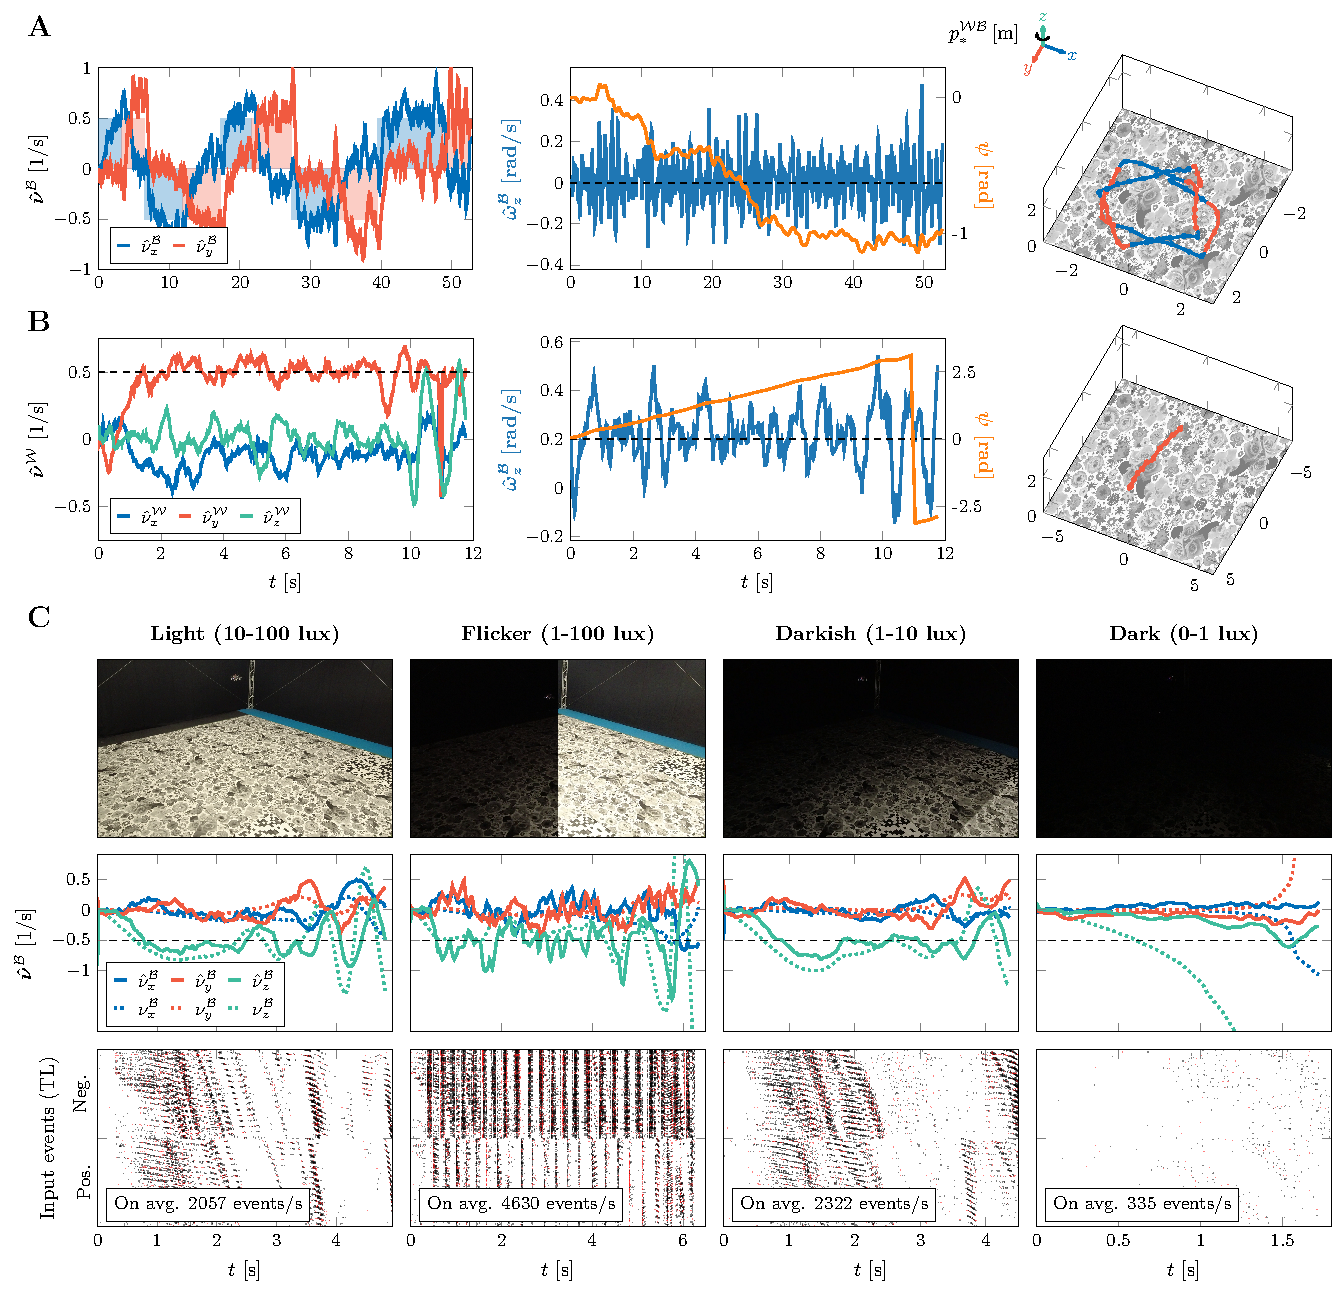
\includegraphics[width=\textwidth]{04_chapters/SR23/figures/fig6-pispecial-results.pdf}
	\caption{Additional results with vision network and proportional-integral (PI) controller. (\textit{A}) \textit{Top row}: alternating setpoints in X and Y (shaded areas) in order to fly a square. \textit{Bottom row}: rotating the scaled velocity setpoint by the yaw angle, while maintaining a yaw rate setpoint of 0.2 rad/s (dashed line), leads to the drone spinning around its Z-axis while flying in a straight line. (\textit{B}) Landing experiments with different lighting conditions. While flickering lights lead to many more events, visual observable estimates (and hence control) only diverge when it is so dark that there are almost no events.}
	\label{fig:sr_results3}
\end{figure*}

Although our main goal is to show a functional fully neuromorphic vision-to-control pipeline, for a broader applicability of this technology it is informative to study the pipeline's robustness and versatility to conditions not encountered during learning. \figref{fig:results3} shows the results for these tests for the combination of the vision-based state estimation and linear network controller. \figref{fig:results3}A displays the user alternating through different unscaled velocity setpoints in X and Y (while keeping yaw constant) in order to let the drone fly a square. Apart from one section, the controller was able to reach the desired setpoint quite quickly, allowing for sharp corners, while keeping yaw drift small (0.06~rad).

Furthermore, we have tested the robustness to lighting conditions for maneuvers in different directions. Here, we show the results of these experiments for the landing maneuver (see Supplementary Results for the other directions). Because landing involves a wider range of visual motion magnitudes than horizontal flight (flow inversely proportional to height), it allowed us to better see the effect of lower-light conditions. Furthermore, divergence-based landings inherently lead to oscillations~\cite{decroon2016monocular}, which makes for a more challenging scenario in the case of flickering lights. \figref{fig:results3}B shows landing with divergence $\nu^\mathcal{B}_{z,\mathrm{sp}}=-0.5$~1/s for various lighting conditions (quantified with lux measurements). With these experiments we aimed to investigate the robustness of the approach to wildly varying event statistics. For instance, in a darker environment, contrasts are less visible, which means that motion will generate many fewer events and that there will be more spurious, noisy events\textemdash similar to our own human vision when we walk in the dark. When lights are switched on and off, this generates massive numbers of events that are unrelated to motion, hence violating the brightness constancy assumption underlying optical flow determination. The events for the top left corner ROI are shown in \figref{fig:results3}B. The results in the light and darkish settings look alike, but flickering lights led to a large increase in events, and the darkest setting gave almost no events. As \figref{fig:results3}B shows, despite the challenging light conditions, the controller was able to track the setpoint (black dashed line) quite well, and the estimated unscaled velocities approximated their ground truths. Only the darkest setting posed a real problem for the state estimation: in that case, the estimated unscaled velocities $\boldsymbol{\hat{\nu}}^\mathcal{B}$ diverged too much from the ground truth unscaled velocities $\boldsymbol{{\nu}}^\mathcal{B}$ to perform a successful landing. %For comparison, the flickering, darkness, and squares experiments have also been performed with the PI controller, which can be found in the Supplementary Results.

Lastly, to demonstrate that successful real-world flight transfers to textures other than those the vision network was trained on, we performed additional tests on other textured surfaces, as shown in \figref{fig_sr:snntexture}. Oscillations in unscaled velocities were similar to those observed above the training texture. %Variations in density of the input events may have been a result of these oscillations or of the texture density.

\begin{figure}[!t]
	\centering
	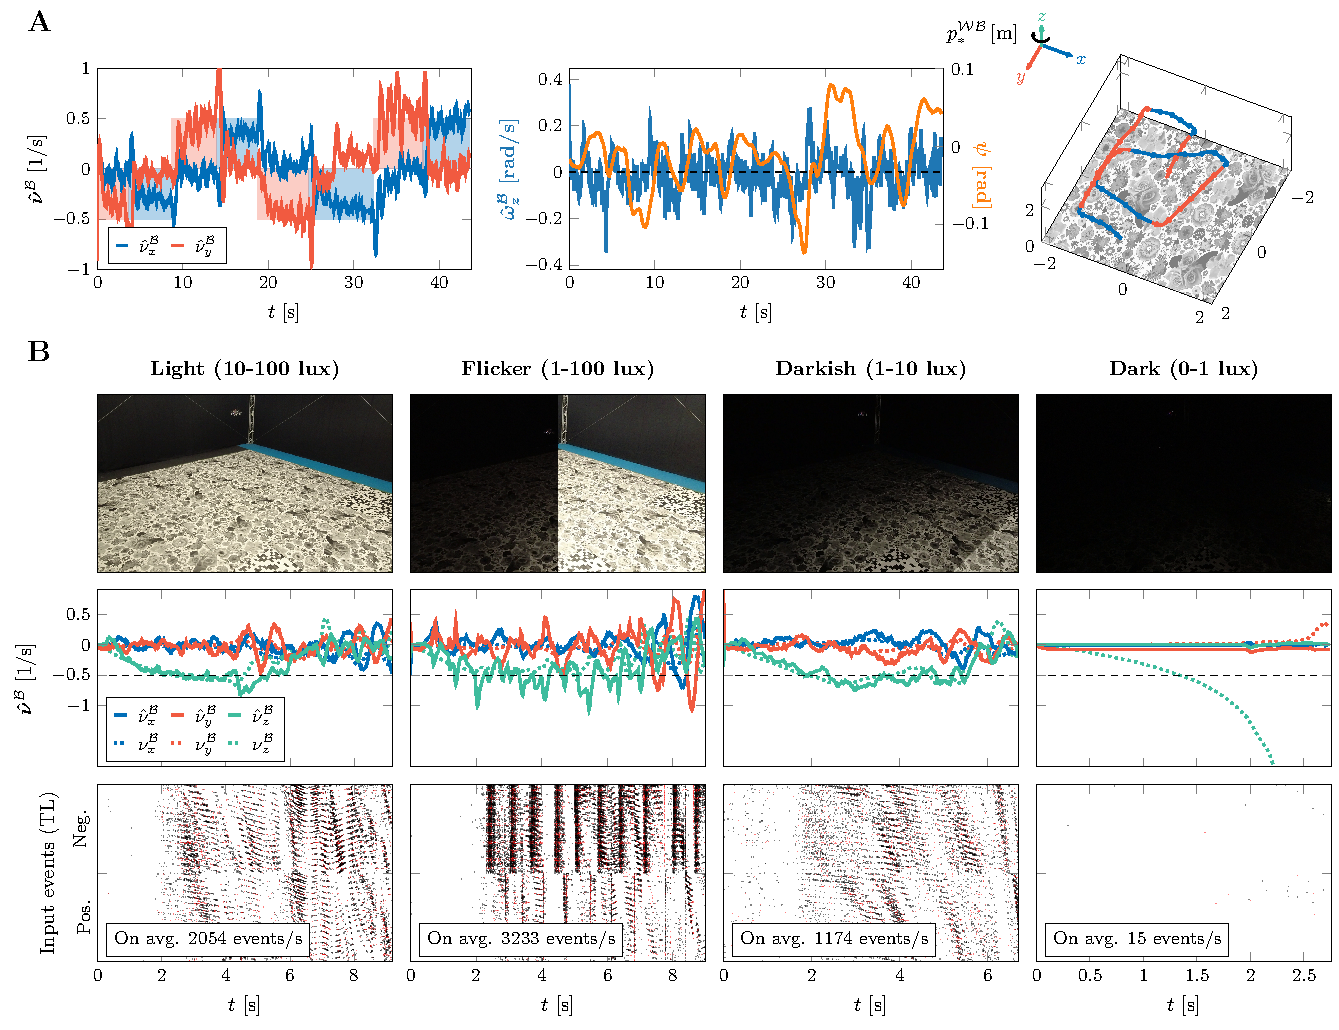
\includegraphics[width=\textwidth]{04_chapters/SR23/figures/fig9-snnspecial-results.pdf}
	\caption{Additional results with vision network and linear network controller. (\textit{A}) Alternating setpoints in X and Y (shaded areas) in order to fly a square. (\textit{B}) Landing experiments with different lighting conditions. While flickering lights lead to many more events, visual observable estimates (and hence control) only diverge when it is so dark that there are almost no events.}
	\label{fig:sr_snnspecial}
\end{figure}


\begin{figure}[!t]
	\centering
	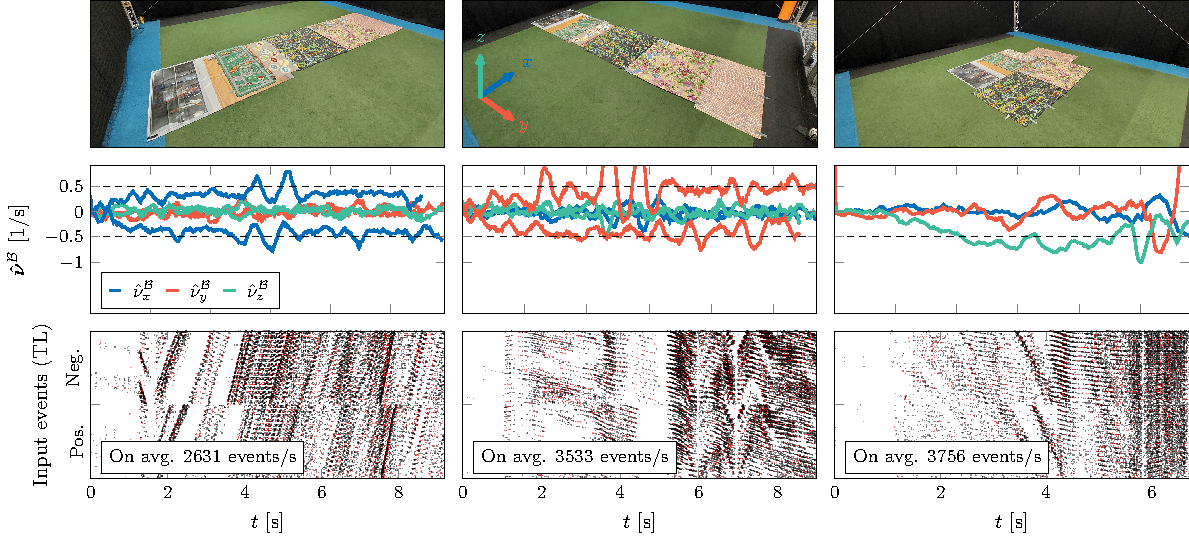
\includegraphics[width=\textwidth]{04_chapters/SR23/figures/fig8-snntexture-results.pdf}
	\caption{Results with vision network and linear network controller for various textures. Flight tests in X, Y and Z over variously textured mats show that the vision network is able to estimate optical flow regardless of texture. Input events are for the $\smash{\nu^\mathcal{B}_{\{x,y\},\mathrm{sp}} = 0.5}$~1/s and $\smash{\nu^\mathcal{B}_{z,\mathrm{sp}} = -0.5}$~1/s tests. Dashed lines show the nonzero setpoints in the motion axis.}
	\label{fig:sr_snntexture}
\end{figure}

\subsection{Benchmarking inference speed and energy consumption}

\begin{table*}[!t]
	\centering
	\resizebox{\textwidth}{!}{%
		\begin{tabular}{@{}lrrrrrrrr@{}}
			\thickhline
			\thickhline
			&  Seq.   & Static [W] & Dynamic [W] & Idle [W] & Running [W] & Delta [W] & inf/s & mJ/inf \\ \midrule
			Nahuku 32 (empty)                      & any    & 0.86      & 0.04       & 0.90    & 0.90       & 4\,e-3     & 60496 & 71\,e-6      \\ \midrule
			\multirow{3}{*}{Nahuku 32: SNN} & slow   & 0.90      & 0.05       & 0.94    & 0.95       & 12\,e-3     & 1637  & 7\,e-3      \\
			& medium & 0.90      & 0.04       & 0.94    & 0.95       & 8\,e-3     & 411   & 21\,e-3     \\
			& fast   & 0.90      & 0.04       & 0.94    & 0.95       & 7\,e-3     & 274   & 27\,e-3     \\ \midrule
			\multirow{3}{*}{Jetson Nano: SNN (5W)}      & slow   & -          & -           & 1.05  & 2.23       & 1.18     & 14     & 86.11 \\
			& medium & -          & -           & 1.03   & 2.25       & 1.22     & 14     & 85.58 \\
			& fast   & -          & -           & 1.03    & 2.24       & 1.21     & 14     & 86.19 \\ \midrule
			\multirow{3}{*}{Jetson Nano: SNN (10W)}     & slow   & -          & -           &  1.04   & 2.98       & 1.93     & 26     & 75.25 \\
			& medium & -          & -           &  1.06   & 2.98       & 1.92     & 26     & 75.35 \\
			& fast   & -          & -           &  1.04   & 2.99       & 1.95     & 25     & 76.52 \\ \midrule
			\multirow{3}{*}{Jetson Nano: ANN (5W)}      & slow   & -          & -           & 1.05  & 2.66       & 1.61     & 59     & 27.46 \\
			& medium & -          & -           & 1.07   & 2.64       & 1.57     & 56     & 27.91 \\
			& fast   & -          & -           & 1.06    & 2.64       & 1.58     & 57     & 27.52 \\ \midrule
			\multirow{3}{*}{Jetson Nano: ANN (10W)}     & slow   & -          & -           &  1.04   & 3.30       & 2.27     & 83     & 27.36 \\
			& medium & -          & -           &  1.07   & 3.33       & 2.26     & 80     & 28.09 \\
			& fast   & -          & -           &  1.07   & 3.30       & 2.23     & 80     & 27.80 \\ 
			\thickhline
			\thickhline
		\end{tabular}
	}
    \caption{Approximate energy and power characteristics for various devices on three sequences: slow, medium and fast. On average, slow has 28.6 events/inf, medium has 106.9 events/inf, and fast has 186.6 events/inf. Delta power is the difference between idle and running (total) power, and was used to compute energy per inference. Dynamic power is the power needed for switching and short-circuiting, and static power is due to leakage; together they sum to running (total) power as well. Nahuku is a board with 32 Loihi chips (Kapoho Bay has 2). A Nahuku configuration where no spikes were sent and only chips and cores were allocated (no synapses) is included as `empty'. Jetson Nano has a low-power (5W) and high-power (10W) mode. One inference (inf) was the processing of one set of inputs by the network, resulting in an output or prediction. On Jetson Nano, we tested both our vision SNN as well as the comparable Conv-GRU ANN.}
	\label{tab:sr_energy}
\end{table*}

\tabref{tab:energy} shows a comparison in terms of power/energy and runtime between the Loihi neuromorphic processor and an NVIDIA Jetson Nano for running the vision network (both SNN as well as equivalent ANN) on sequences with varying amounts of motion and hence varying input event density. The SNN ran in hardware on Loihi and in software (PyTorch) on Jetson Nano. The tests for Loihi were performed on a Nahuku board, which contains 32 Loihi chips. We confirmed, insofar possible, that using two chips on Nahuku is representative of a Kapoho Bay (at least in terms of execution time), which is the two-chip form factor used on the drone. Still, neither of these benchmarks is completely representative of the tests performed in the real world: the benchmarks used data already loaded in memory, and therefore only quantified the processing by the network without any bottlenecks due to input/output (I/O) and preprocessing, whereas the flight tests involved streaming event data that was coming in and was being processed in an online fashion. This showed in Loihi's execution frequencies in \tabref{tab:energy}, which were well above the 200 inferences (with one inference being the processing of one set of inputs by the network) per second (inf/s) achieved during flight tests.

\tabref{tab:energy} shows the power when the processors were idle and when they were running the networks. Because Jetson Nano does not provide static and dynamic power components, we compared the difference between idle and running power, and used that to compute energy per inference. A main observation is that the Nahuku 32 board consumed 0.95~W when running the SNN, whereas Jetson Nano consumed $\sim$2.98~W when running in 10W mode. This is a difference of a factor $\sim $3.1$\times$. Most of the energy expenditure of Loihi consisted of idle power. \tabref{tab:energy} also shows the difference between the idle power and the power when running the network (`Delta'). When only considering this extra power required for the inference of the network, Loihi outperformed Jetson Nano by three to four orders of magnitude, depending on the sequence. Hence, any possible reduction of the idle power would substantially affect the neuromorphic chip's energy efficiency advantages over other chips. 

Moreover, Loihi provided a one to two orders of magnitude improvement in execution frequency. Furthermore, the benefits of neuromorphic processing show in Loihi's increasing execution frequency as event sparsity increased (from fast to slow motion sequences).
Because a GPU like Jetson Nano is not optimized to simulate SNNs, we also ran an equivalent ANN (Conv-GRU with downsampling, corner crop ROI and event limiting from \tabref{tab:sr_AEEchanges}). The increased inference speed for the ANN on Jetson Nano confirms that this is indeed a more suitable architecture for GPUs. Nonetheless, although energy consumption per inference has decreased compared to running the SNN on Jetson Nano, energy efficiency and inference speed still did not come close to those of the SNN on Loihi.

\section{Conclusion}

We presented a fully neuromorphic vision-to-control pipeline for controlling a flying drone. Specifically, we trained a spiking neural network that takes in raw event-based camera data and produces low-level control commands. Real-world experiments demonstrated a successful sim-to-real transfer: the drone can accurately follow various ego-motion setpoints, performing hovering, landing, and lateral maneuvers\textemdash even under constant yaw rate. 

Our study confirms the potential of a fully neuromorphic vision-to-control pipeline by running on board with an execution frequency of 200~Hz. Moreover, the chip spends 0.95~W, out of which 0.94~W is idle power and only 7-12~mW is used for inference. Hence, reducing the idle power can lead to substantial energy gains. 

A major question is whether the energy gain of neuromorphic processing will make a difference on a system level even if future neuromorphic chips weigh in the order of grams and will have a negligible idle power. Compared to the power required for hovering, 277~W, a difference of a few watts (see \tabref{tab:energy}) may seem like a small difference. However, on flying robots, such small differences can have substantial effects \cite{boroujerdian2018mavbench}. A heavier, more power-consuming computing unit does not only require more power from the battery, but it also needs to be lifted in the air. This requires a bigger battery and possibly bigger motors that themselves also have to be lifted. Moreover, as argued in \cite{boroujerdian2018mavbench}, a lower latency, as attained with neuromorphic processing, allows for faster flight. This in turn leads to drones accomplishing their missions with less flight time. Still, the main point is not necessarily what you gain on a $\sim$1-kilogram drone if you switch from a conventional embedded GPU to a lightweight neuromorphic processor (which is not negligible), but that neuromorphic processing will enable many more networks to run on such larger drones and even enable deep neural networks on much lighter platforms that cannot even carry an embedded GPU. An example of the latter are 30-gram flapping wing drones, which use $\sim$6~W to fly\cite{karasek2018tailless}. 

A particularly promising avenue to autonomous flight of such tiny drones is to make the entire drone sensing, processing, and actuation pipeline neuromorphic, from its accelerometer sensors to the processor and motors, allowing for sparse and event-driven/asynchronous computation all the way through. Because such hardware is currently not available, we have limited ourselves to the vision-to-control pipeline, ending at thrust and attitude commands.

Until then, advancements could come from improved I/O bandwidth and interfacing options for the neuromorphic processor and event camera. The current processor is limited to host boards with an x86 architecture (preventing other potentially lighter but equally performant architectures from being used), and can only be connected directly via AER to a specific model of event-based camera (this is of course also a limitation on the part of the available event cameras). Although the former is limiting for all works implementing neuromorphic hardware on constrained systems like drones, the latter is especially relevant to our advanced use case, where we reached the limits of the number of spikes that can be sent to and received from the neuromorphic processor at the desired high execution frequency of 200~Hz. To achieve this frequency, we had to limit the number of events per input window to 90 per image corner ROI, and limit ourselves to a linear network controller, which avoids having to send additional input spikes that encode the ego-motion setpoint and attitude. Improved interfacing could allow for more extensive vision processing and more complex spiking neuron control networks. This could make the vision-based ego-motion estimation more robust and considerably increase the control performance\textemdash even if spiking neural network controllers currently perform worse than common PID controllers \cite{stagsted2020event,stroobants2022design}. Please note that as long as both the vision and control networks still use a learned encoding and decoding the proposed split-and-merge strategy would still work (see Materials and Methods). 
Ultimately, further gains in terms of efficiency might be obtained by moving from digital neuromorphic processors to mixed-signal hardware, but this will pose even larger development and deployment challenges given the noise sensitivity of such hardware \cite{sandamirskaya2022neuromorphic,frenkel2023bottomup}.

Despite the above-mentioned limitations, the current work presents a substantial step towards neuromorphic sensing and processing for drones. The results are encouraging, because they show that neuromorphic sensing and processing may bring deep neural networks within reach of small autonomous robots. In time this may allow them to approach the agility, versatility and robustness of small animals such as flying insects.

\section*{Supplementary material}
\vspace{10pt}
%\begin{itemize}
%	\setlength\itemsep{0.5em}
%	\item Video playlist of the approach: \textbf{TODO}
%%	\item Project code: \textbf{TODO}
%\end{itemize}

\newlist{mylist_sr}{itemize}{1}
\setlist[mylist_sr]{label=\hspace{0pt}}
\newcommand\itemonesr{\item \qrcode[height=0.4in]{https://www.youtube.com/playlist?list=PL_KSX9GOn2P-pyEODPVIb6PXfjr4BXuqH}}

\begin{mylist_sr}[leftmargin=*, align=left, leftmargin=2em, itemindent=0pt, labelsep=0pt, labelwidth=2em]
	\itemonesr\quad Video playlist of the approach: \url{https://tinyurl.com/4edsypye}
\end{mylist_sr}